% =========================================================
% ARTIST PORTFOLIO TEMPLATE
% ---------------------------------------------------------
% Populate this template by running:
%   python generate_portfolio.py --template portfolio_template.tex \
%                                --data portfolio_data.json \
%                                --output portfolio.pdf
%
% The script replaces %%PLACEHOLDER%% markers with values
% from the JSON data file and filesystem project metadata.
%
% Compile with xelatex (required for fontspec).
% =========================================================

\documentclass[12pt]{article}

% ---------------------------------------------------------
% PAGE LAYOUT
% ---------------------------------------------------------
\usepackage[a4paper, landscape, margin=0.8in, headheight=22pt, headsep=14pt]{geometry}

% ---------------------------------------------------------
% PACKAGES
% ---------------------------------------------------------
\usepackage{graphicx}     % image inclusion
\usepackage{float}        % figure placement [H]
\usepackage{titlesec}     % section styling
\usepackage{fancyhdr}     % headers / footers
\usepackage{parskip}      % no paragraph indent, space between paragraphs
\usepackage{caption}      % captions
\usepackage{tabularx}     % flexible tables
\usepackage{hyperref}     % links
\usepackage{xcolor}
\usepackage{wrapfig}      % text wrapping around figures
\usepackage{tikz}         % full-page label overlay
% SVGs are pre-converted to PDF by the Python generator (rsvg-convert)
\usepackage{fontspec}     % requires xelatex

\usepackage{setspace}
\setstretch{1.6}

% ---------------------------------------------------------
% TYPOGRAPHY
% ---------------------------------------------------------
% Montserrat from local folder
\setmainfont{Montserrat}[
    Path           = montserrat/,
    UprightFont    = *-Light,
    BoldFont       = *-SemiBold,
    ItalicFont     = *-LightItalic,
    BoldItalicFont = *-SemiBoldItalic,
    Extension      = .ttf
]

% ---------------------------------------------------------
% HYPERLINK STYLE
% ---------------------------------------------------------
\hypersetup{
    colorlinks = true,
    linkcolor  = black,
    urlcolor   = black,
}

% ---------------------------------------------------------
% HEADER / FOOTER
% ---------------------------------------------------------
\pagestyle{fancy}
\fancyhf{}
\fancyhead[L]{\small {\addfontfeature{LetterSpace=8}\href{https://patriciogonzalezvivo.com}{\MakeUppercase{Patricio Gonzalez Vivo}}}}
\fancyhead[R]{\footnotesize \rightmark}
\renewcommand{\headrulewidth}{1pt}

% ---------------------------------------------------------
% SECTION STYLE
% ---------------------------------------------------------
\titleformat{\section}
  {\Large\bfseries}{}
  {0pt}{}[\titlerule]

\titleformat{\subsection}
  {\large\bfseries}{}
  {0pt}{}

% ---------------------------------------------------------
% ARTWORK MACRO
% ---------------------------------------------------------
% Parameters:
%   #1 = image path
%   #2 = title
%   #3 = year
%   #4 = medium
%   #5 = dimensions
%   #6 = description
%
% The script generates \ArtworkEntry calls for each project.

\newcommand{\ArtworkEntry}[6]{

\clearpage

\begin{center}

\includegraphics[width=0.9\textwidth,height=0.85\textheight,keepaspectratio]{#1}

\vspace{1em}

{\Large \textbf{#2}}

\vspace{0.5em}

\begin{tabular}{rl}
Year:       & #3 \\
Medium:     & #4 \\
Dimensions: & #5 \\
\end{tabular}

\end{center}

\vspace{1em}

#6

}

% ---------------------------------------------------------
% SERIES DIVIDER MACRO
% ---------------------------------------------------------
\newcommand{\SeriesPage}[1]{
\clearpage
\begin{center}
\vspace*{0.3\textheight}
{\Huge \textbf{#1}}
\end{center}
\clearpage
}

% =========================================================
% DOCUMENT START
% =========================================================
\begin{document}

\thispagestyle{empty}
\begin{tikzpicture}[overlay, remember picture]
  \node[anchor=center] at (current page.center) {%
    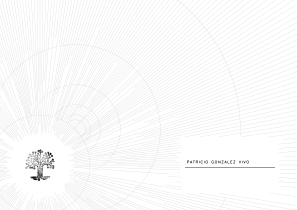
\includegraphics[width=\paperwidth,height=\paperheight]{portfolio/label_output.pdf}%
  };
\end{tikzpicture}
\clearpage

% % ---------------------------------------------------------
% % COVER PAGE
% % ---------------------------------------------------------
% \thispagestyle{empty}

% \begin{center}

% \vspace*{3cm}

% 
\includegraphics[width=2cm]{images/logo-gray.png}

% {\LARGE \textbf{Patricio Gonzalez Vivo}}

% {\Large %%PORTFOLIO_TITLE%%}

% \vfill

% \href{mailto:patriciogonzalezvivo@gmail.com}{patriciogonzalezvivo@gmail.com}

% \href{https://patriciogonzalezvivo.com}{patriciogonzalezvivo.com}

% \end{center}

% \clearpage

\markright{Bio}
\textbf{Patricio Gonzalez Vivo} (b. 1982, Buenos Aires) is a multidisciplinary artist working across traditional and digital media. He explores awareness, perception, and self-discovery through motifs such as celestial artifacts, esoteric symbolism, and temporal cartographies. His work weaves together the poetic and the procedural, revealing hidden structures behind the ways we measure and make sense of the world.

\begin{wrapfigure}{r}{0.40\textwidth}
\vspace{-\intextsep}
\href{https://patriciogonzalezvivo.com/2011/efectomariposa/}{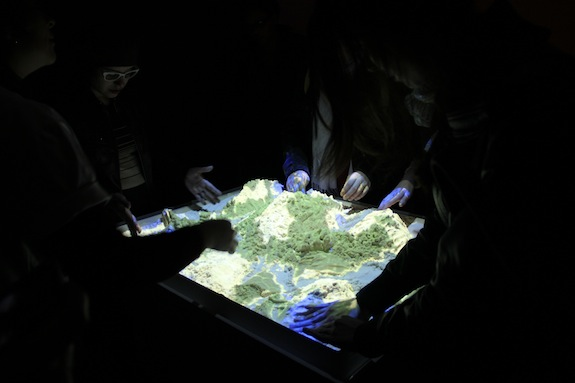
\includegraphics[width=\linewidth,keepaspectratio]{2011/efectomariposa/images/12.jpg}}
\par\vspace{0.4em}
{\small \raggedleft
\textbf{Efecto Mariposa}, 2011 \\
FILE Festival, São Paulo
\par}
\vspace{-\intextsep}
\end{wrapfigure}


Originally trained in clinical psychology and expressive arts therapy, Patricio's early works centered on participatory installations designed to foster the experience of collective co-creation. One of his first major work, \href{https://patriciogonzalezvivo.com/2010/communitas/}{\textbf{Communitas (2010)}}, invited visitors to collaboratively construct a shared image through mutual observation and gesture. His first international breakthrough, \href{https://patriciogonzalezvivo.com/2011/efectomariposa/}{\textbf{Efecto Mariposa (2011)}}, was an ash-based installation that simulated an interactive ecosystem in which visitors experienced the cascading consequences of their actions. These projects examined the tensions between chaos and order, the individual, and the collective, the ephemeral, and the enduring.

In 2012, he relocated to the United States to pursue an MFA in Design \& Technology at Parsons School of Design. During this period, his practice shifted toward the construction of algorithmic tools and custom creative systems like: \href{https://www.patriciogonzalezvivo.com/2014/skylines/skylines.php?v=01}{\textbf{drawing machines}}, \href{https://patriciogonzalezvivo.com/tools.php}{\textbf{live-coding environments, open-source libraries}}, some of which are still the buildings blocks of his practice. Since 2017, he has expanded this research through the creation of his own astronomical instruments, exploring the relationship between inner experience and the cosmos through scale, time, and presence.

In more recent years, and particularly in response to the proliferation of machine-generated imagery, Patricio has returned to traditional oil painting, not as a rejection of technology, but as a way of insisting on something machines cannot replicate: the slow accumulation of attention, the risk of failure, the presence of a body in time. For Patricio, human intelligence is fundamentally embodied, it emerges through sensation, intuition, and lived experience, and this conviction shapes every dimension of his practice. 

\begin{wrapfigure}{l}{0.40\textwidth}
\vspace{-\intextsep}
\href{https://pixelspiritdeck.com}{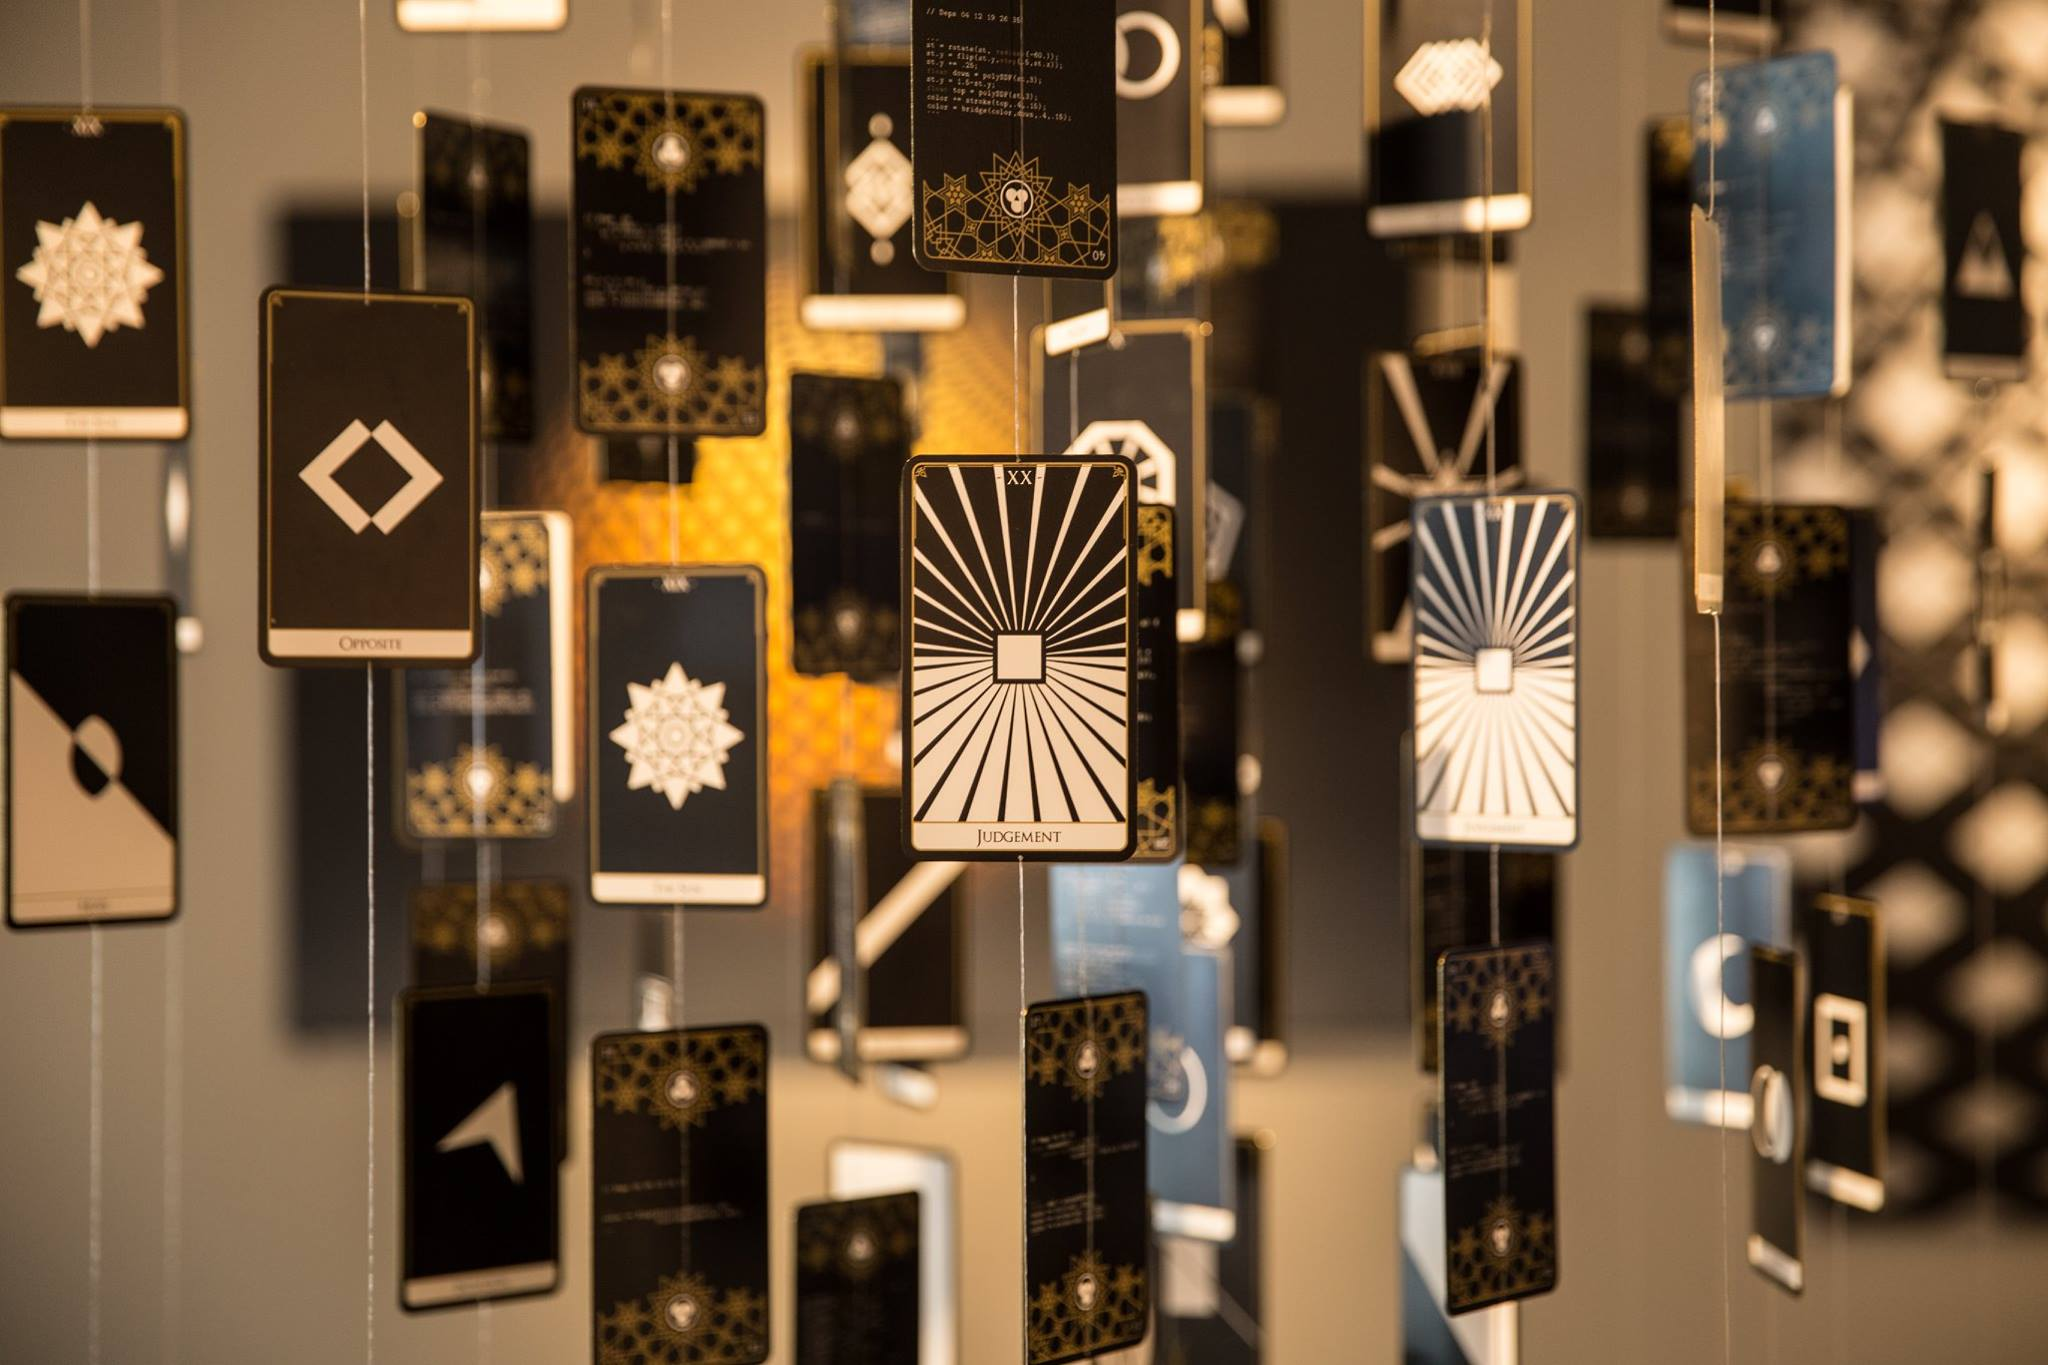
\includegraphics[width=\linewidth,keepaspectratio]{2017/pixelspirit/images/22383968_1665365133488191_5147193364633286006_o.jpg}}
\par\vspace{0.4em}
{\small \raggedright
\textbf{Pixel Spirit}, 2017 \\
Tarot Deck, 50 cards, 4.75 x 2.5 inches each
\par}
\vspace{-\intextsep}
\end{wrapfigure}


A defining commitment of Patricio's work is open dissemination. He develops and releases open-source libraries and platforms that expand the possibilities of digital art, positioning software as both a medium for knowledge and for expression. His influential \href{https://thebookofshaders.com/}{\textbf{Book of Shaders (2015)}} become a foundational resource for digital artists working. Similarly his \href{https://patriciogonzalezvivo.com/www.pixelspiritdeck.com}{\textbf{PixelSpirit tarot Deck (2017)}}, which bridges the ancient divination system with shader programming, it's another education tool that bridges the poetic nature of code with esoteric knowledge. Patricio also shares openly his digital building blocks in the form of libraries such as \href{https://github.com/patriciogonzalezvivo/lygia}{\textbf{Lygia}}, \href{https://github.com/patriciogonzalezvivo/vera}{\textbf{Vera}}, \href{https://github.com/patriciogonzalezvivo/berthe}{\textbf{Berthe}}, and \href{https://github.com/patriciogonzalezvivo/hypatia}{\textbf{Hypatia}}, which are ongoing as instruments for creative exploration. For the artist, this open sharing is not ancillary to the work, it is itself a form of authorship and cultural contribution.

His work has been exhibited and presented internationally at platforms such as \href{http://eyeofestival.com/}{\textbf{EYEO}}, \href{http://resonate.io/}{\textbf{Resonate}}, \href{https://www.grow.paris/}{\textbf{GROW}}, \href{http://file.org.br/}{\textbf{FILE}}, \href{http://espacio.fundaciontelefonica.com/}{\textbf{Espacio Fundación Telefónica}}, \href{https://www.brightmoments.io/}{\textbf{BrightMoments}}, \href{https://youtu.be/aIjeF9QgH-Q}{\textbf{FlyingTokyo}}, \href{https://www.dotdotdot.it/conn/graphics-machine-learning-patricio.php}{\textbf{DotDotDot}} and \href{http://encuentrofase.com.ar/}{\textbf{FASE}}. He has delivered talks and lectures at institutions including the \href{https://www.media.mit.edu/}{\textbf{MIT Media Lab}}, \href{https://www.cmu.edu/cfa/studio/}{\textbf{Carnegie Mellon University, Frank-Ratchye Studio for Creative Inquiry}} and Politecnico di Milano. He has taught at \href{http://www.newschool.edu/parsons/mfa-design-technology/}{\textbf{Parsons School of Design}}, \href{http://tisch.nyu.edu/itp}{\textbf{ITP NYU}}, \href{http://sfpc.io/}{\textbf{SFPC (School for Poetic Computation)}}, and the Instituto Universitario Nacional de Arte in Argentina.
\vspace{3em}
\begin{center}

\includegraphics[height=2cm,keepaspectratio]{images/logo-gray.png}
\end{center}


\clearpage

\markright{Artist Statement}

\section*{Artist Statement}

For years I built computational systems: drawing machines, generative software, real-time tools that translate structure into image. Now I am also a painter. These are not two practices in conflict — they are two ways of asking the same questions about memory, perception, and what it means to look at another person or place with genuine attention.

My hybrid paintings begin with custom software: a computer vision program analyzes a portrait and translates its structure into vector paths, which a plotter draws onto a primed canvas. What the machine produces is accurate but incomplete — a skeleton, waiting. Then I return with oil and brush. Freed from measurement, I can enter the painting as a space to inhabit rather than to describe. The scaffold is given; the presence is earned.

The same investigation runs through my software works. \textit{Weaver} maps two observers' night skies onto each other to find the stars they hold in common. \textit{BLINK} translates the Baroque vanitas — the soap bubble as memento mori — into a real-time system at planetary scale. These works are not illustrations of ideas. They are systems built to produce a specific kind of encounter: an experience of time, scale, or connection that would not exist otherwise.

What holds across all of it is a single conviction: that intelligence is embodied, that attention is a material, and that making something slowly — with a brush, with code, with a hand-built machine — remains a meaningful act of care.



\clearpage

% ---------------------------------------------------------
% SELECTED WORKS
% ---------------------------------------------------------
% \section*{Selected Works}

\clearpage
\markright{\href{https://patriciogonzalezvivo.com/2026/santos/}{Santos}, 2025-2026}
\noindent{\Large\textbf{\href{https://patriciogonzalezvivo.com/2026/santos/}{Santos}}}\hfill{\large \href{https://patriciogonzalezvivo.com/2025-2026/}{\textcolor{red}{2025-2026}}}

\begin{wrapfigure}{r}{0.40\textwidth}
\vspace{-\intextsep}
\noindent\hfill \href{https://patriciogonzalezvivo.com/2026/santos/}{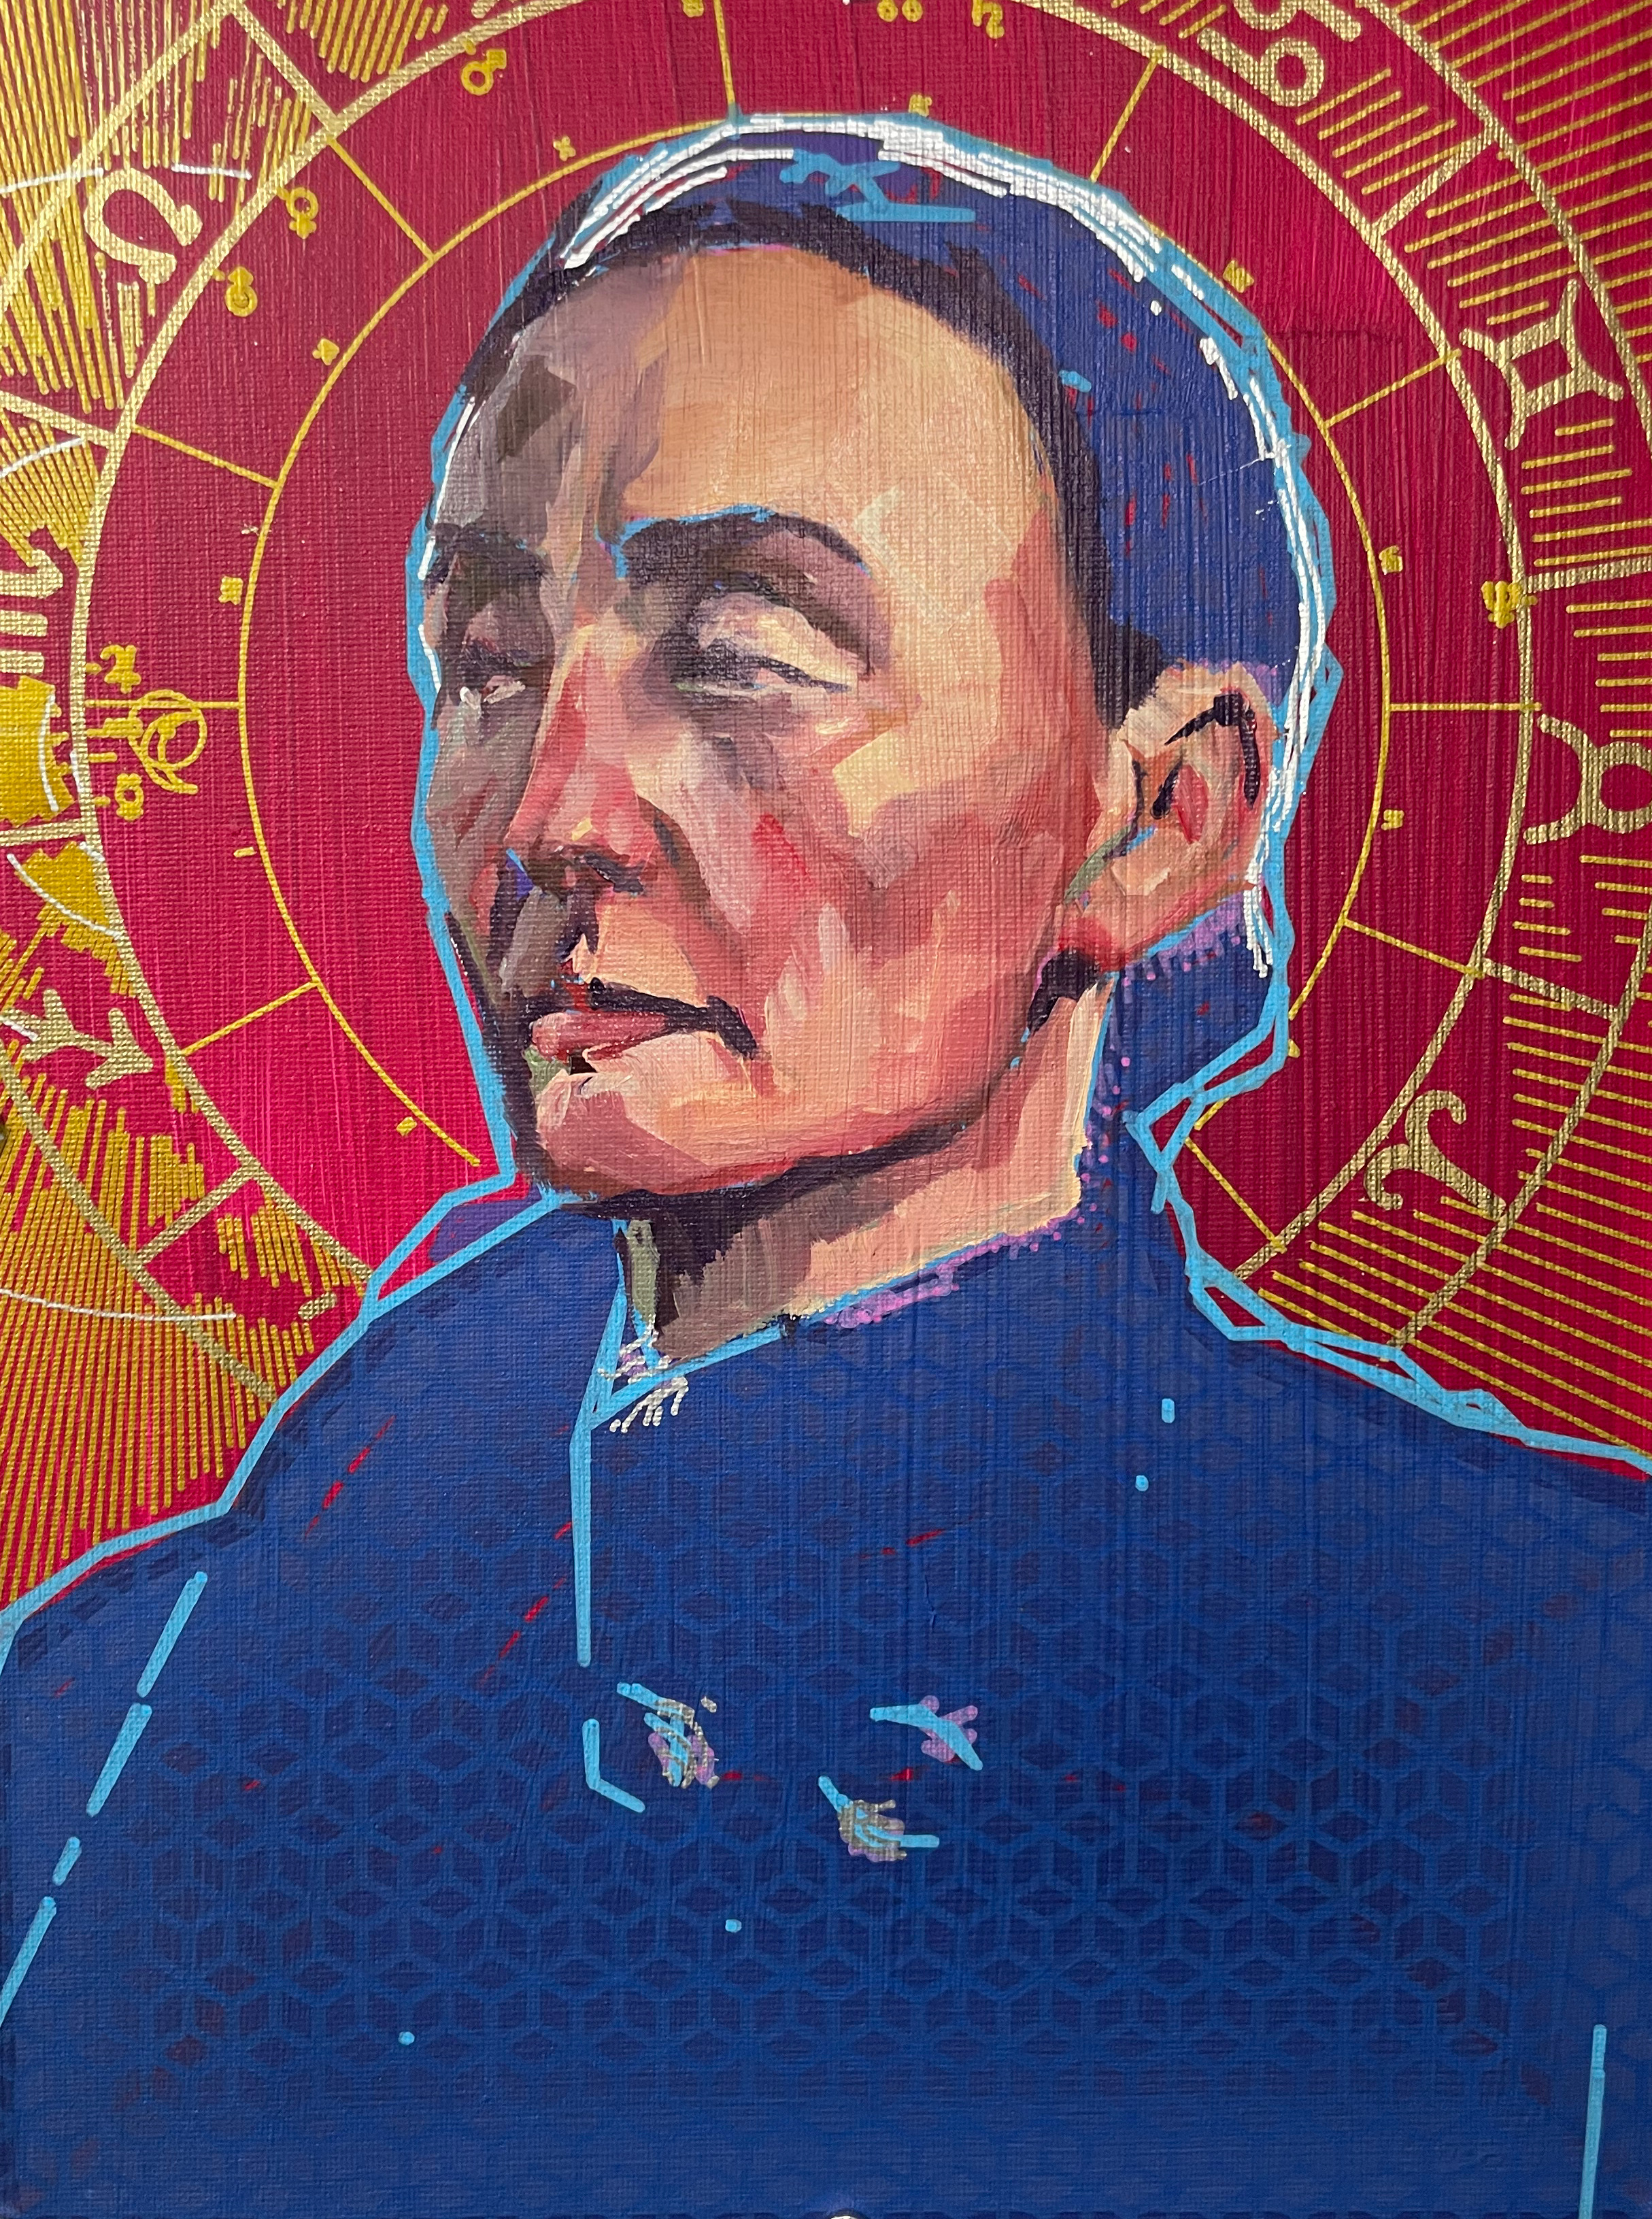
\includegraphics[width=\linewidth,height=0.75\textheight,keepaspectratio]{2026/santos/thumbnail.jpg}}
\vspace{-\intextsep}
\end{wrapfigure}
In Latin America, it is common to receive the name of the saint whose feast day coincides with one's birth. To ask for someone's santo is, in effect, to ask for their birthday. This custom reflects a deep cultural belief: that the saint linked to your day of birth becomes a protector, a guide, and a source of inspiration. Saints, historical figures revered for their moral virtue and spiritual significance, are understood to transcend linear time. Through their acts of compassion and faith, they enter a more circular, mythological temporality, becoming enduring presences within the collective imagination of Christianity.

I was raised in a Catholic family. My grandfather used to read to me from a red book in his study, a compendium of saints' lives. Alongside brief narratives, there were illustrations, each saint marked by a halo, captured at the pivotal moment of transformation when the ordinary gave way to the transcendent. Again and again, these stories returned to a common thread: self-sacrifice, service, and devotion to others. The halo functioned as a visual language for this metaphysical shift.

That ethos of service extended into my family's expectations. Professions such as law, medicine, and engineering were valued as pathways toward a life of usefulness and contribution. In my lineage, I cannot trace a single artist. There is one fragile exception, my maternal great-grandmother, a poet who reportedly burned all her writings upon marriage, as though creativity were a deviation to be corrected, a path to be relinquished in favor of duty.

This series of portraits emerges from a personal search for an alternative lineage, one composed of figures whose service to humanity is enacted through creation. These are individuals committed to the discipline of imagination, capable of translating the invisible into form, and of reshaping the world through beauty, wonder, and possibility.

If there is a creator who invites us into existence as co-creators, then this lineage of artists stands as a kind of secular sainthood. They are not exemplars of moral virtue in the traditional sense, but they are, for me, figures of devotion, visionaries with whom I seek communion and dialogue.

---

\begin{wrapfigure}{l}{0.40\textwidth}
\vspace{-\intextsep}
\href{https://patriciogonzalezvivo.com/2014/skylines/}{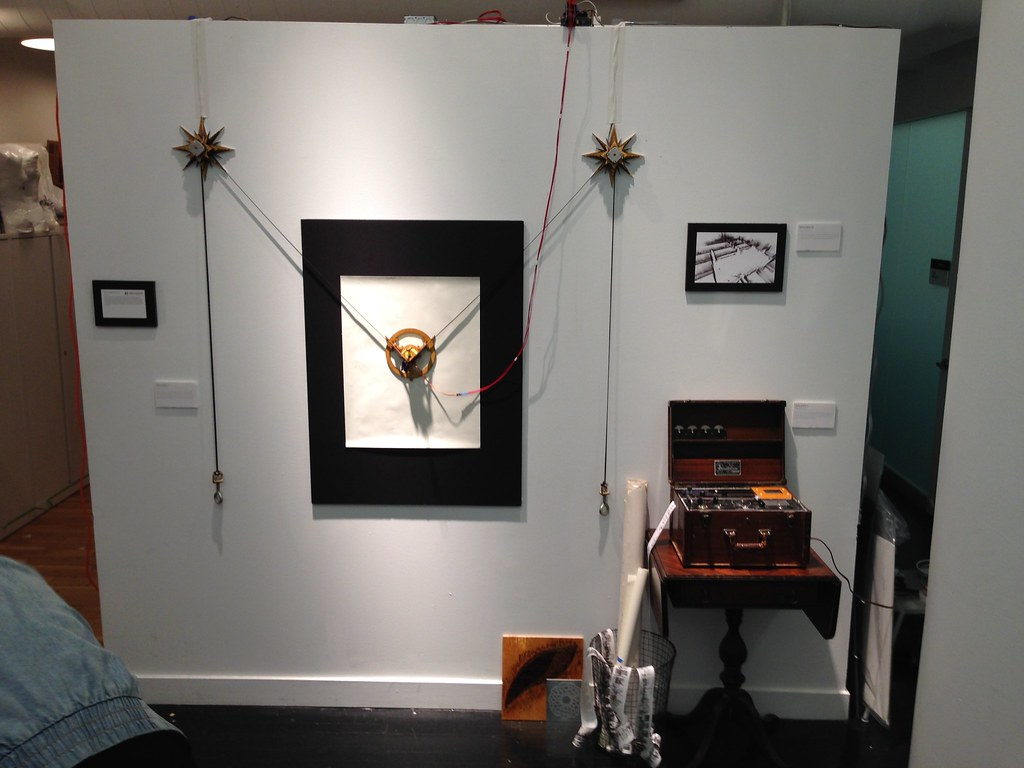
\includegraphics[width=\linewidth,keepaspectratio]{2026/santos/../../2014/skylines/images/14005408208_fbc2fab7ed_b.jpg}}
\par\vspace{0.4em}
{\small \raggedright
\textbf{Skylines}, 2014 \\
Installation detail at gallery
\par}
\vspace{-\intextsep}
\end{wrapfigure}


These portraits continue an exploration of drawing machines begun with \href{https://patriciogonzalezvivo.com/2014/skylines/skylines.php?v=01}{\textbf{Skylines in 2014}}, for which I constructed a wall plotter that slowly reveals an image through custom software translating photographs into lines. In 2025, with the \href{https://patriciogonzalezvivo.com/2025/hybrids/}{\textbf{Hybrids series}}, I began combining plotting with alla prima oil painting, bringing together the forces of machine and hand, code and gesture. In Santos, I use that same approach: converting portrait images into vector paths layered with symbolic elements singular to each subject, plotting the result with acrylic paint on a primed canvas, then completing each portrait by hand with oil.

Like their subjects, the works exist as syntheses: of the material and the immaterial, the earthly and the cosmic, the known and the intuited. They stand as reflections on creativity's enduring capacity to transcend boundaries and connect us to something beyond ourselves.



\begin{center}
  \includegraphics[width=\linewidth]{temp_portfolio/html_renders/html_block_c7a95fbc92ce.png}
\end{center}



\clearpage
{\setlength{\parskip}{0pt}%
\noindent
\begin{minipage}[b][\textheight][b]{0.48\textwidth}
  \hfill\href{https://patriciogonzalezvivo.com/2026/santos/#DSF1035}{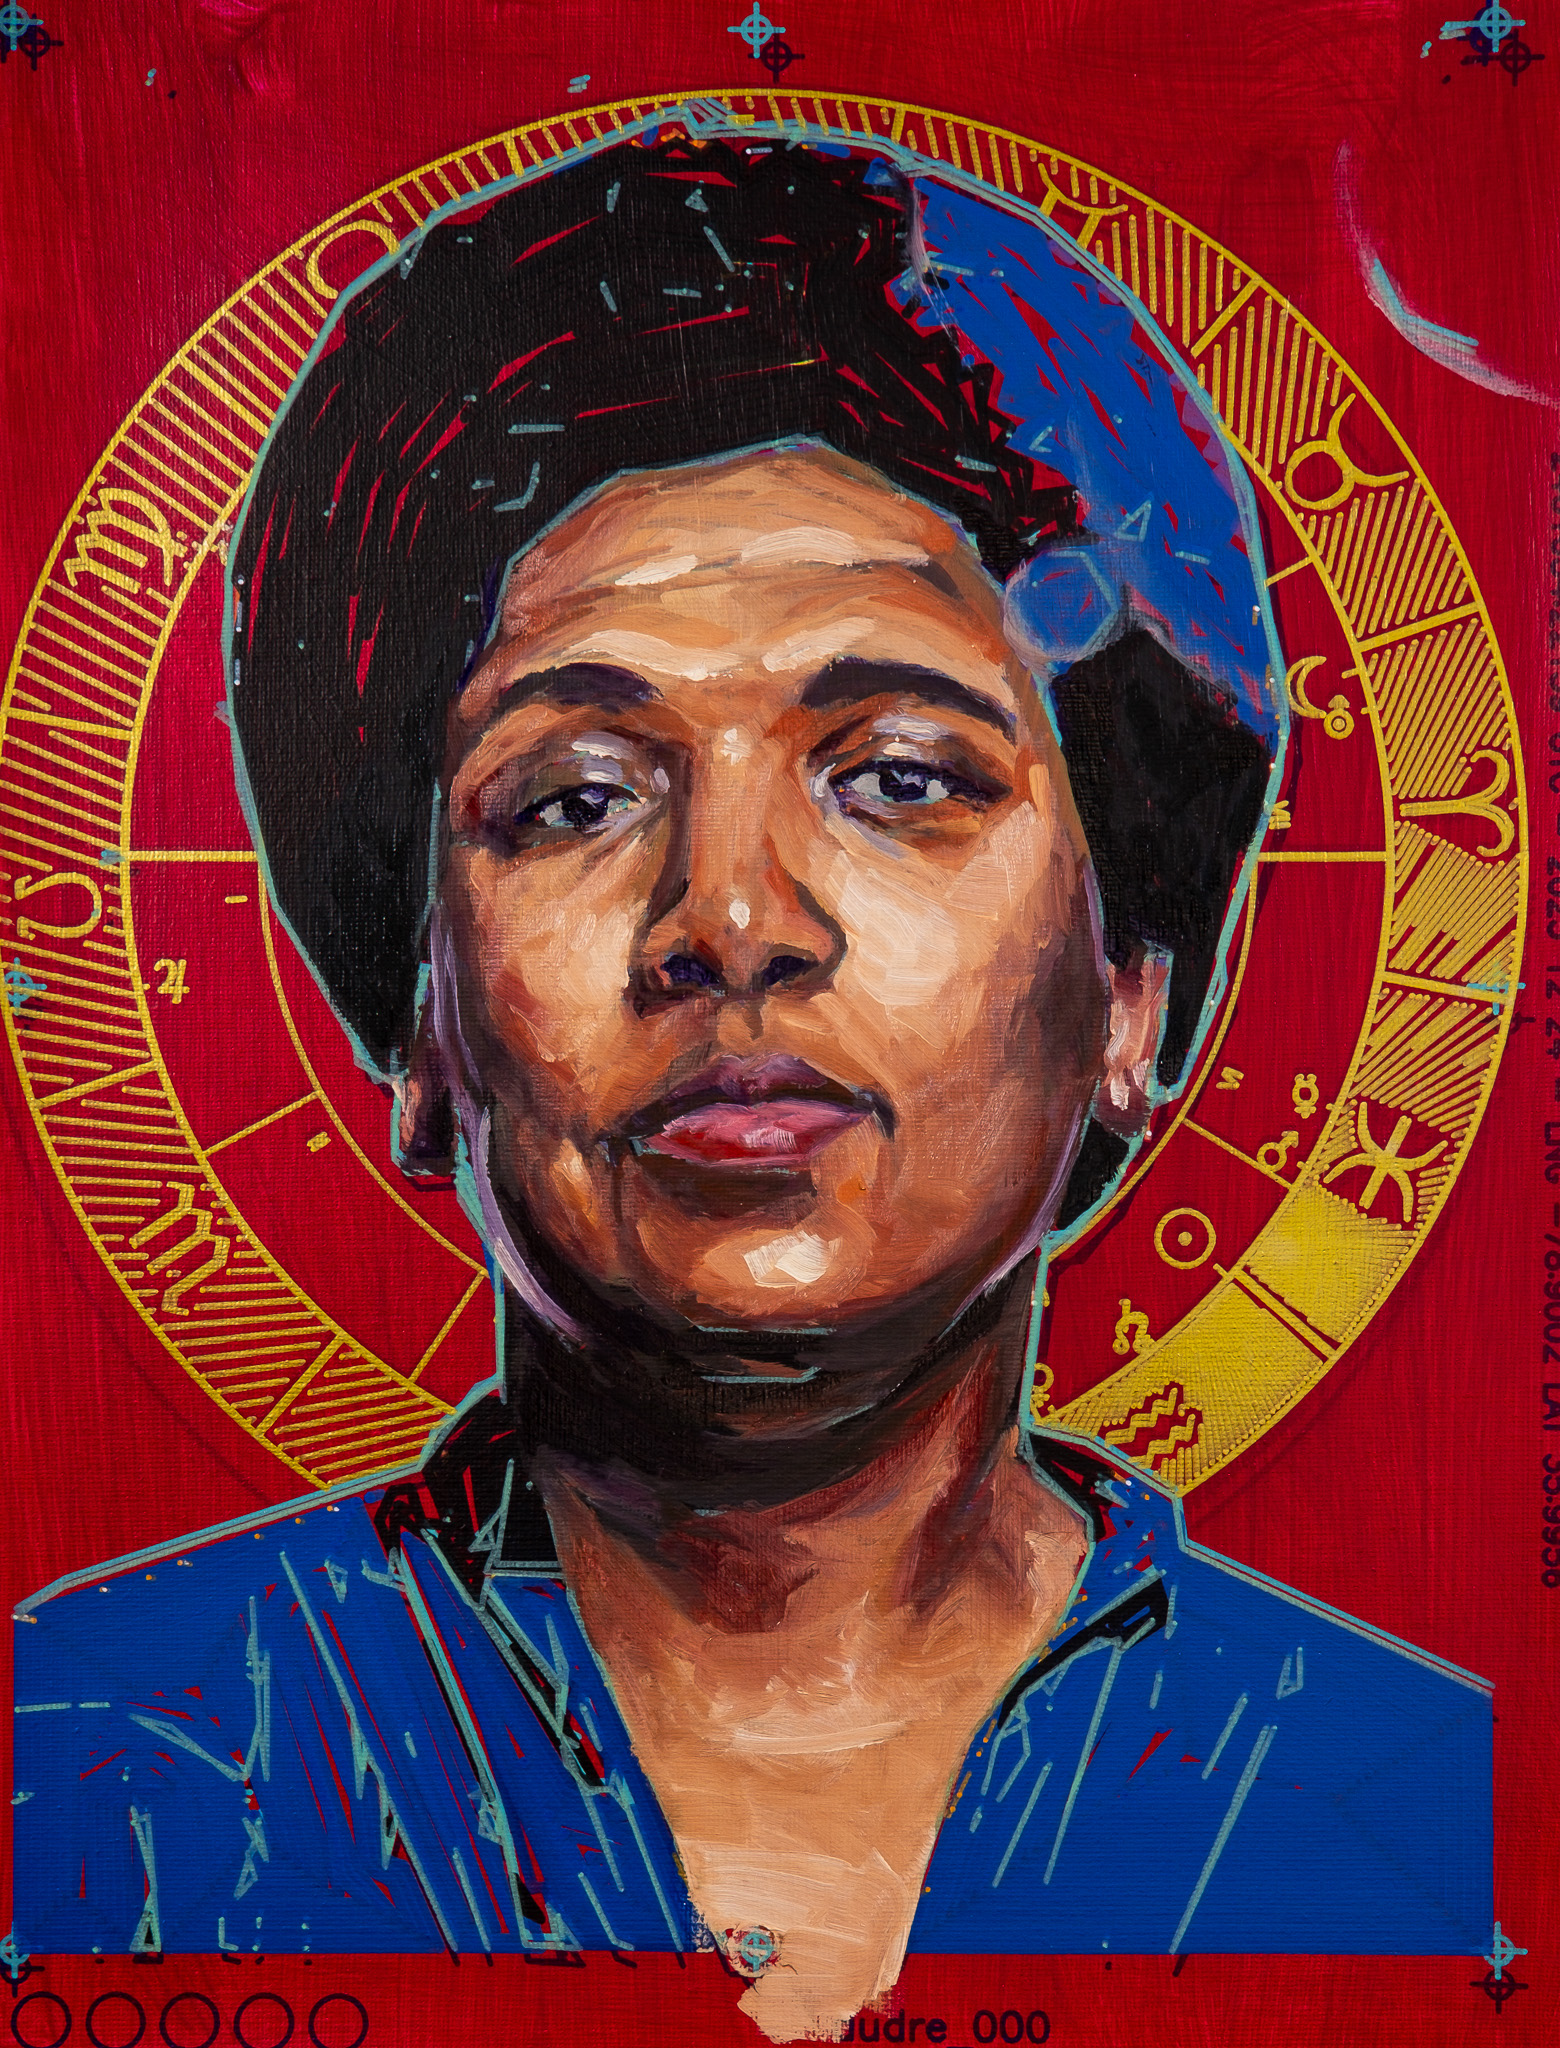
\includegraphics[width=\linewidth,height=\textheight,keepaspectratio]{2026/santos/images/DSF1035.jpg}}
\end{minipage}
\hfill
\begin{minipage}[b][\textheight][b]{0.48\textwidth}
  {\renewcommand{\arraystretch}{1.0}\setstretch{1.0}\selectfont
\begin{tabular}[b]{@{}l@{}}
Audre, 2025\\
Oil on canvas\\
16 x 12 inches
\end{tabular}}
\end{minipage}%
}%
\clearpage
{\setlength{\parskip}{0pt}%
\noindent
\begin{minipage}[b][\textheight][b]{0.48\textwidth}
  \hfill{\renewcommand{\arraystretch}{1.0}\setstretch{1.0}\selectfont
\begin{tabular}[b]{@{}r@{}}
Jorge Luis, 2025\\
Oil on canvas\\
16 x 12 inches
\end{tabular}}
\end{minipage}
\hfill
\begin{minipage}[b][\textheight][b]{0.48\textwidth}
  \href{https://patriciogonzalezvivo.com/2026/santos/#DSF1036}{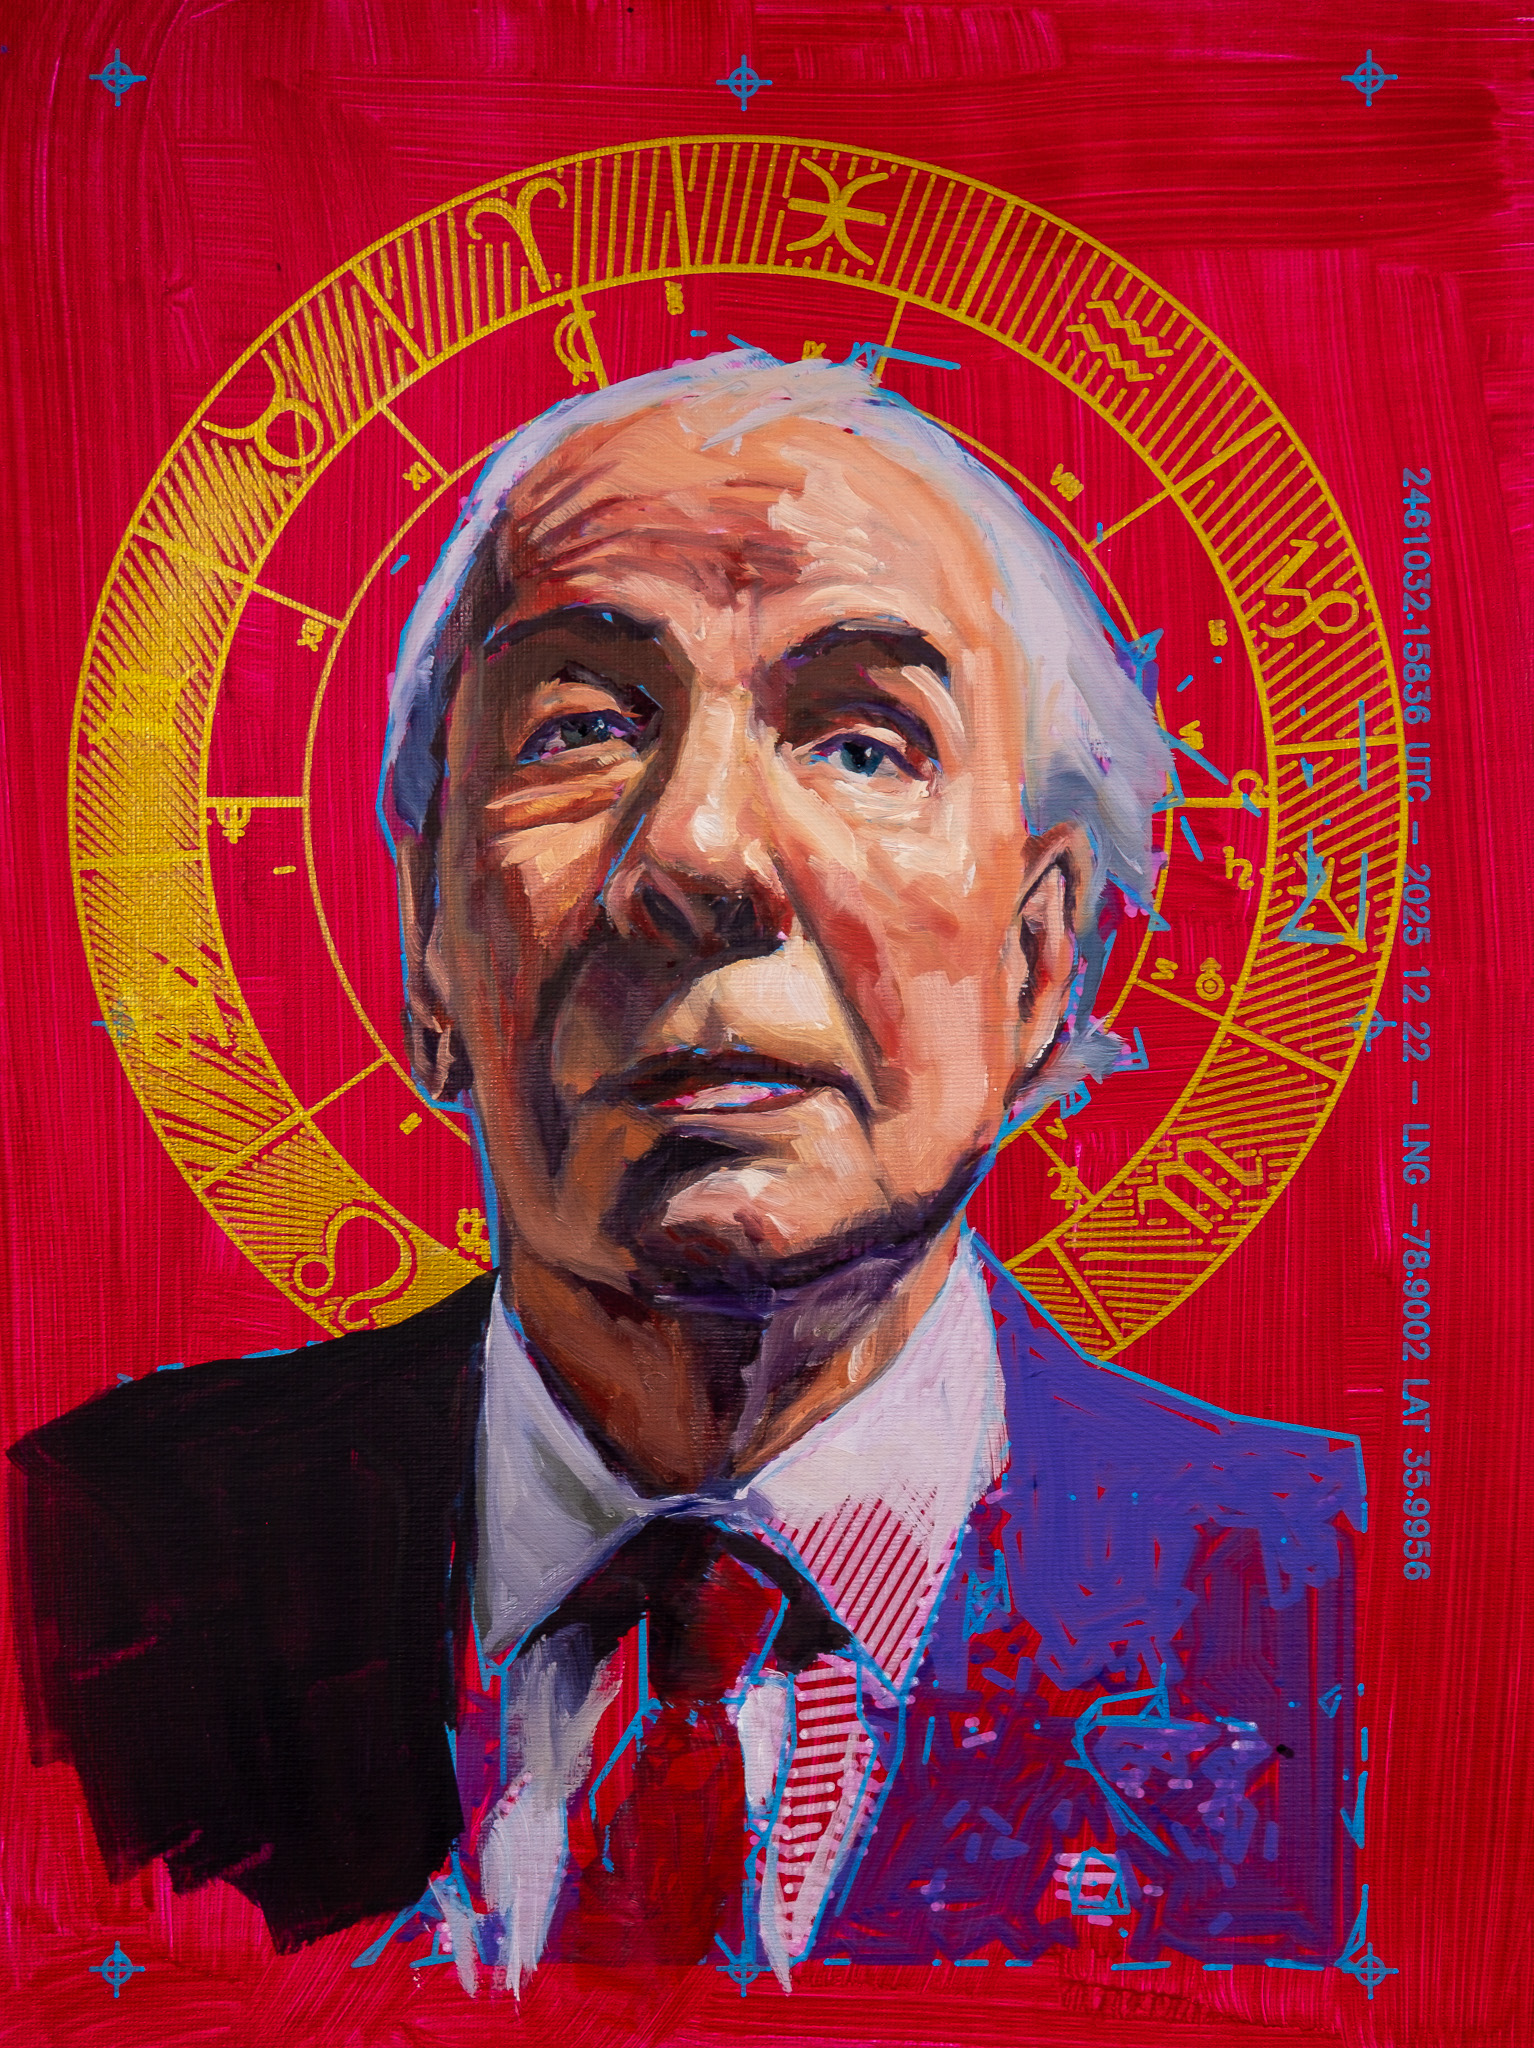
\includegraphics[width=\linewidth,height=\textheight,keepaspectratio]{2026/santos/images/DSF1036.jpg}}
\end{minipage}%
}%
\clearpage
{\setlength{\parskip}{0pt}%
\noindent
\begin{minipage}[b][\textheight][b]{0.48\textwidth}
  \hfill\href{https://patriciogonzalezvivo.com/2026/santos/#DSF1037}{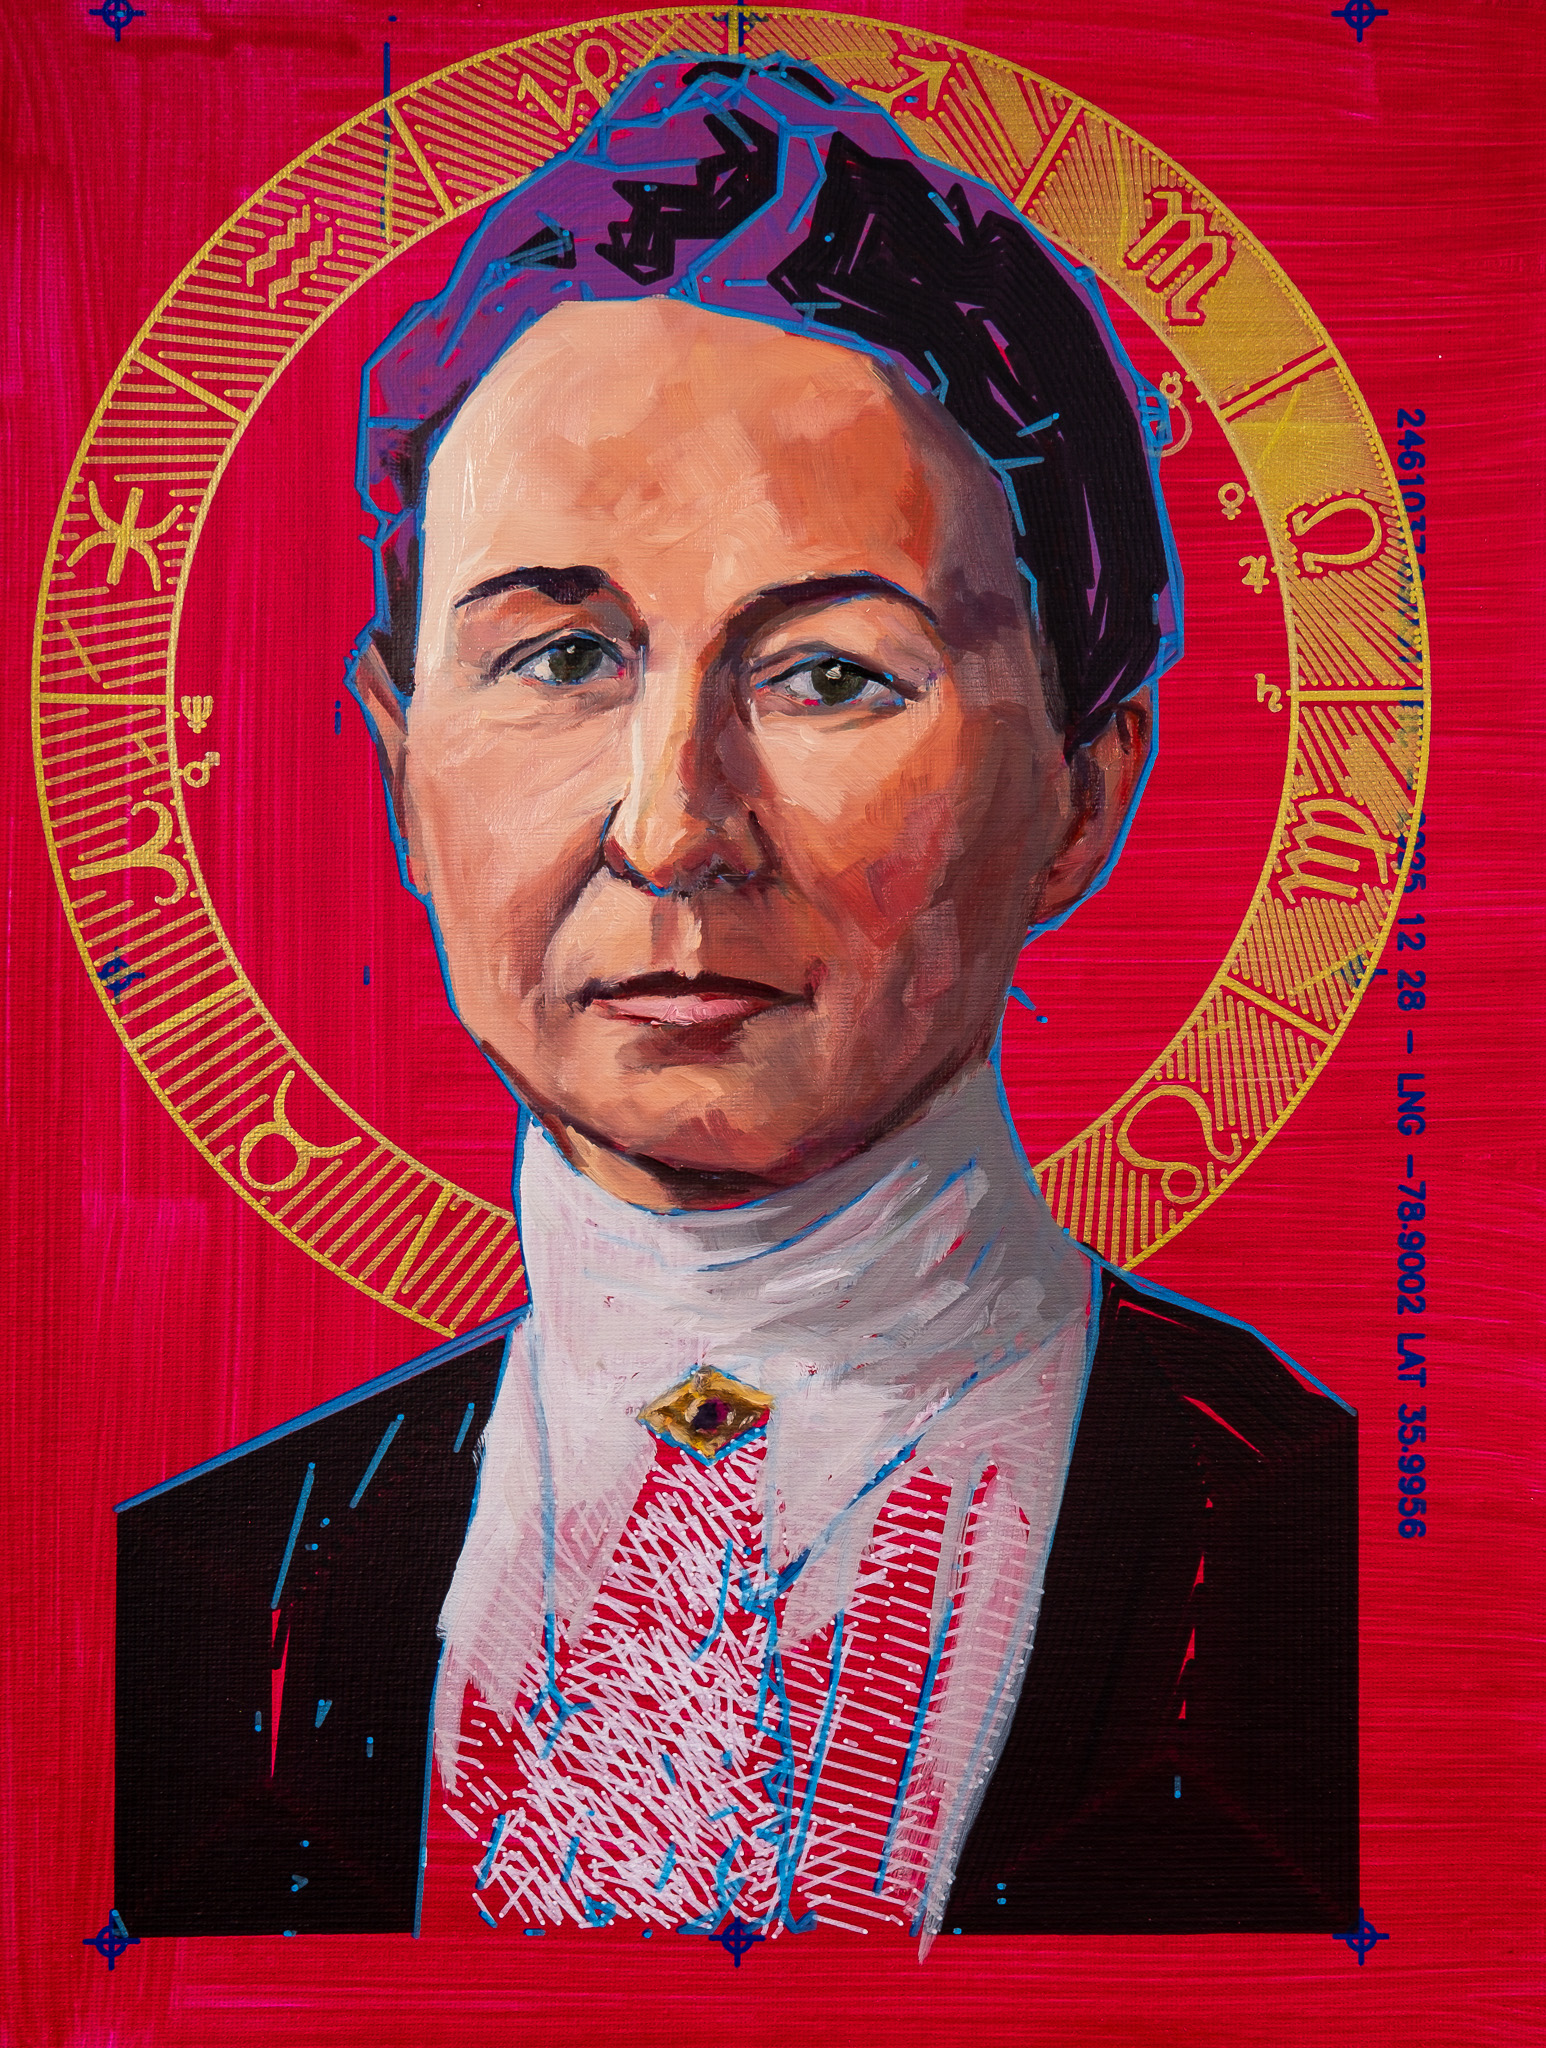
\includegraphics[width=\linewidth,height=\textheight,keepaspectratio]{2026/santos/images/DSF1037.jpg}}
\end{minipage}
\hfill
\begin{minipage}[b][\textheight][b]{0.48\textwidth}
  {\renewcommand{\arraystretch}{1.0}\setstretch{1.0}\selectfont
\begin{tabular}[b]{@{}l@{}}
Hilma, 2025\\
Oil on canvas\\
16 x 12 inches
\end{tabular}}
\end{minipage}%
}%
\clearpage
{\setlength{\parskip}{0pt}%
\noindent
\begin{minipage}[b][\textheight][b]{0.48\textwidth}
  \hfill{\renewcommand{\arraystretch}{1.0}\setstretch{1.0}\selectfont
\begin{tabular}[b]{@{}r@{}}
James, 2025\\
Oil on canvas\\
16 x 12 inches
\end{tabular}}
\end{minipage}
\hfill
\begin{minipage}[b][\textheight][b]{0.48\textwidth}
  \href{https://patriciogonzalezvivo.com/2026/santos/#DSF1038}{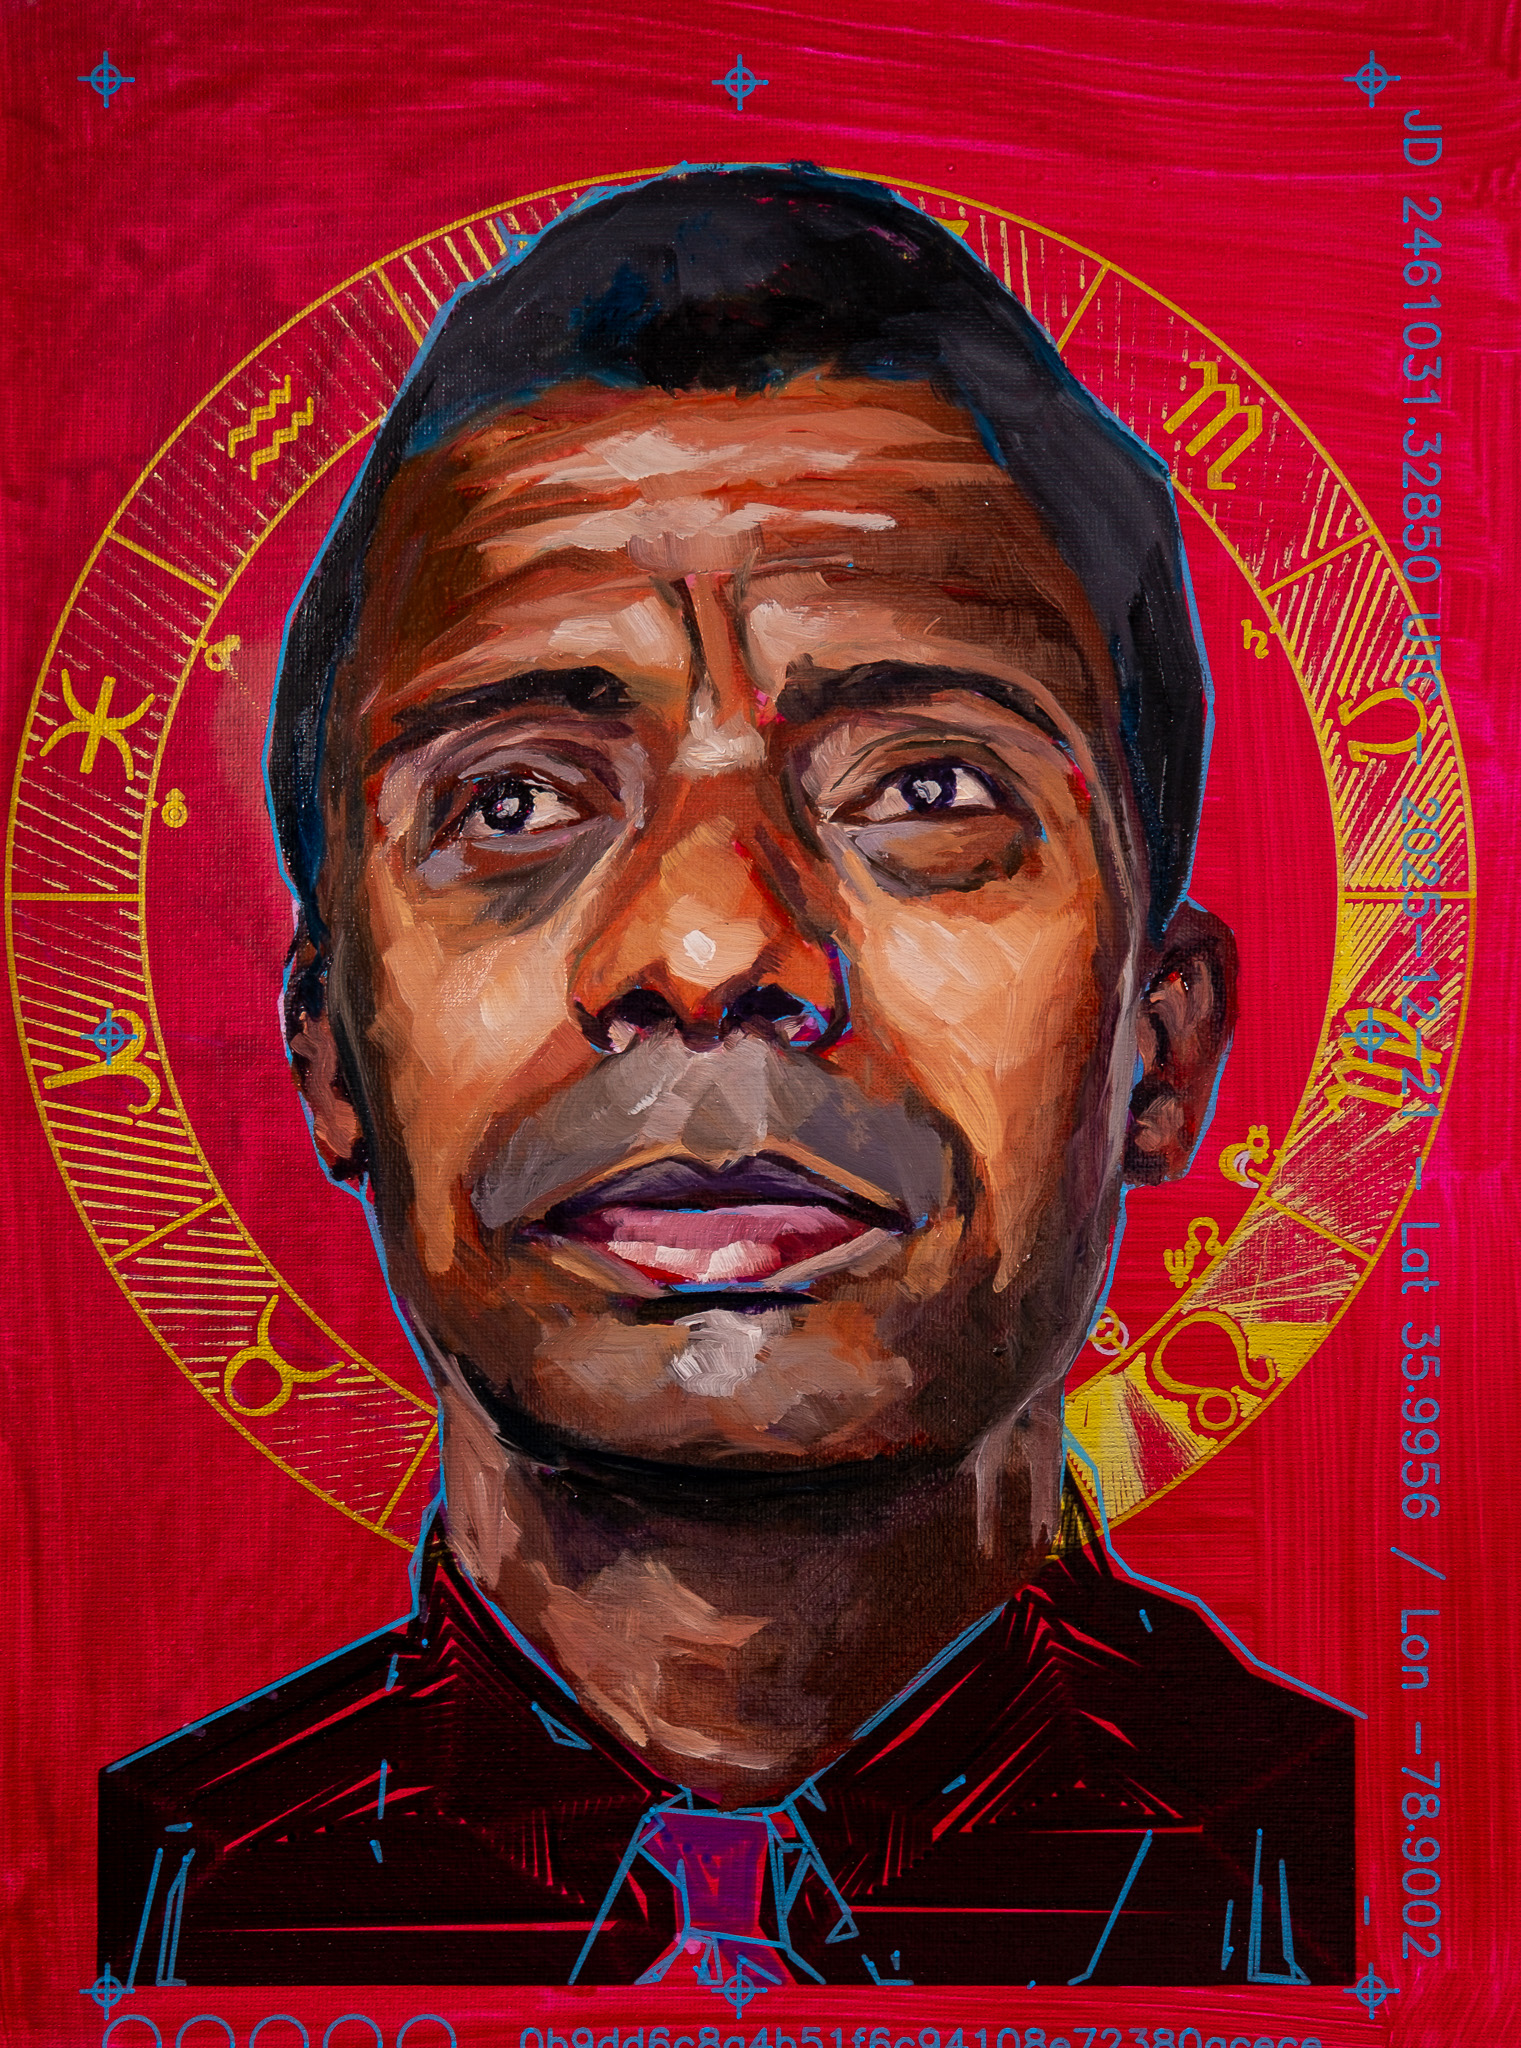
\includegraphics[width=\linewidth,height=\textheight,keepaspectratio]{2026/santos/images/DSF1038.jpg}}
\end{minipage}%
}%
\clearpage
{\setlength{\parskip}{0pt}%
\noindent
\begin{minipage}[b][\textheight][b]{0.48\textwidth}
  \hfill\href{https://patriciogonzalezvivo.com/2026/santos/#DSF1039}{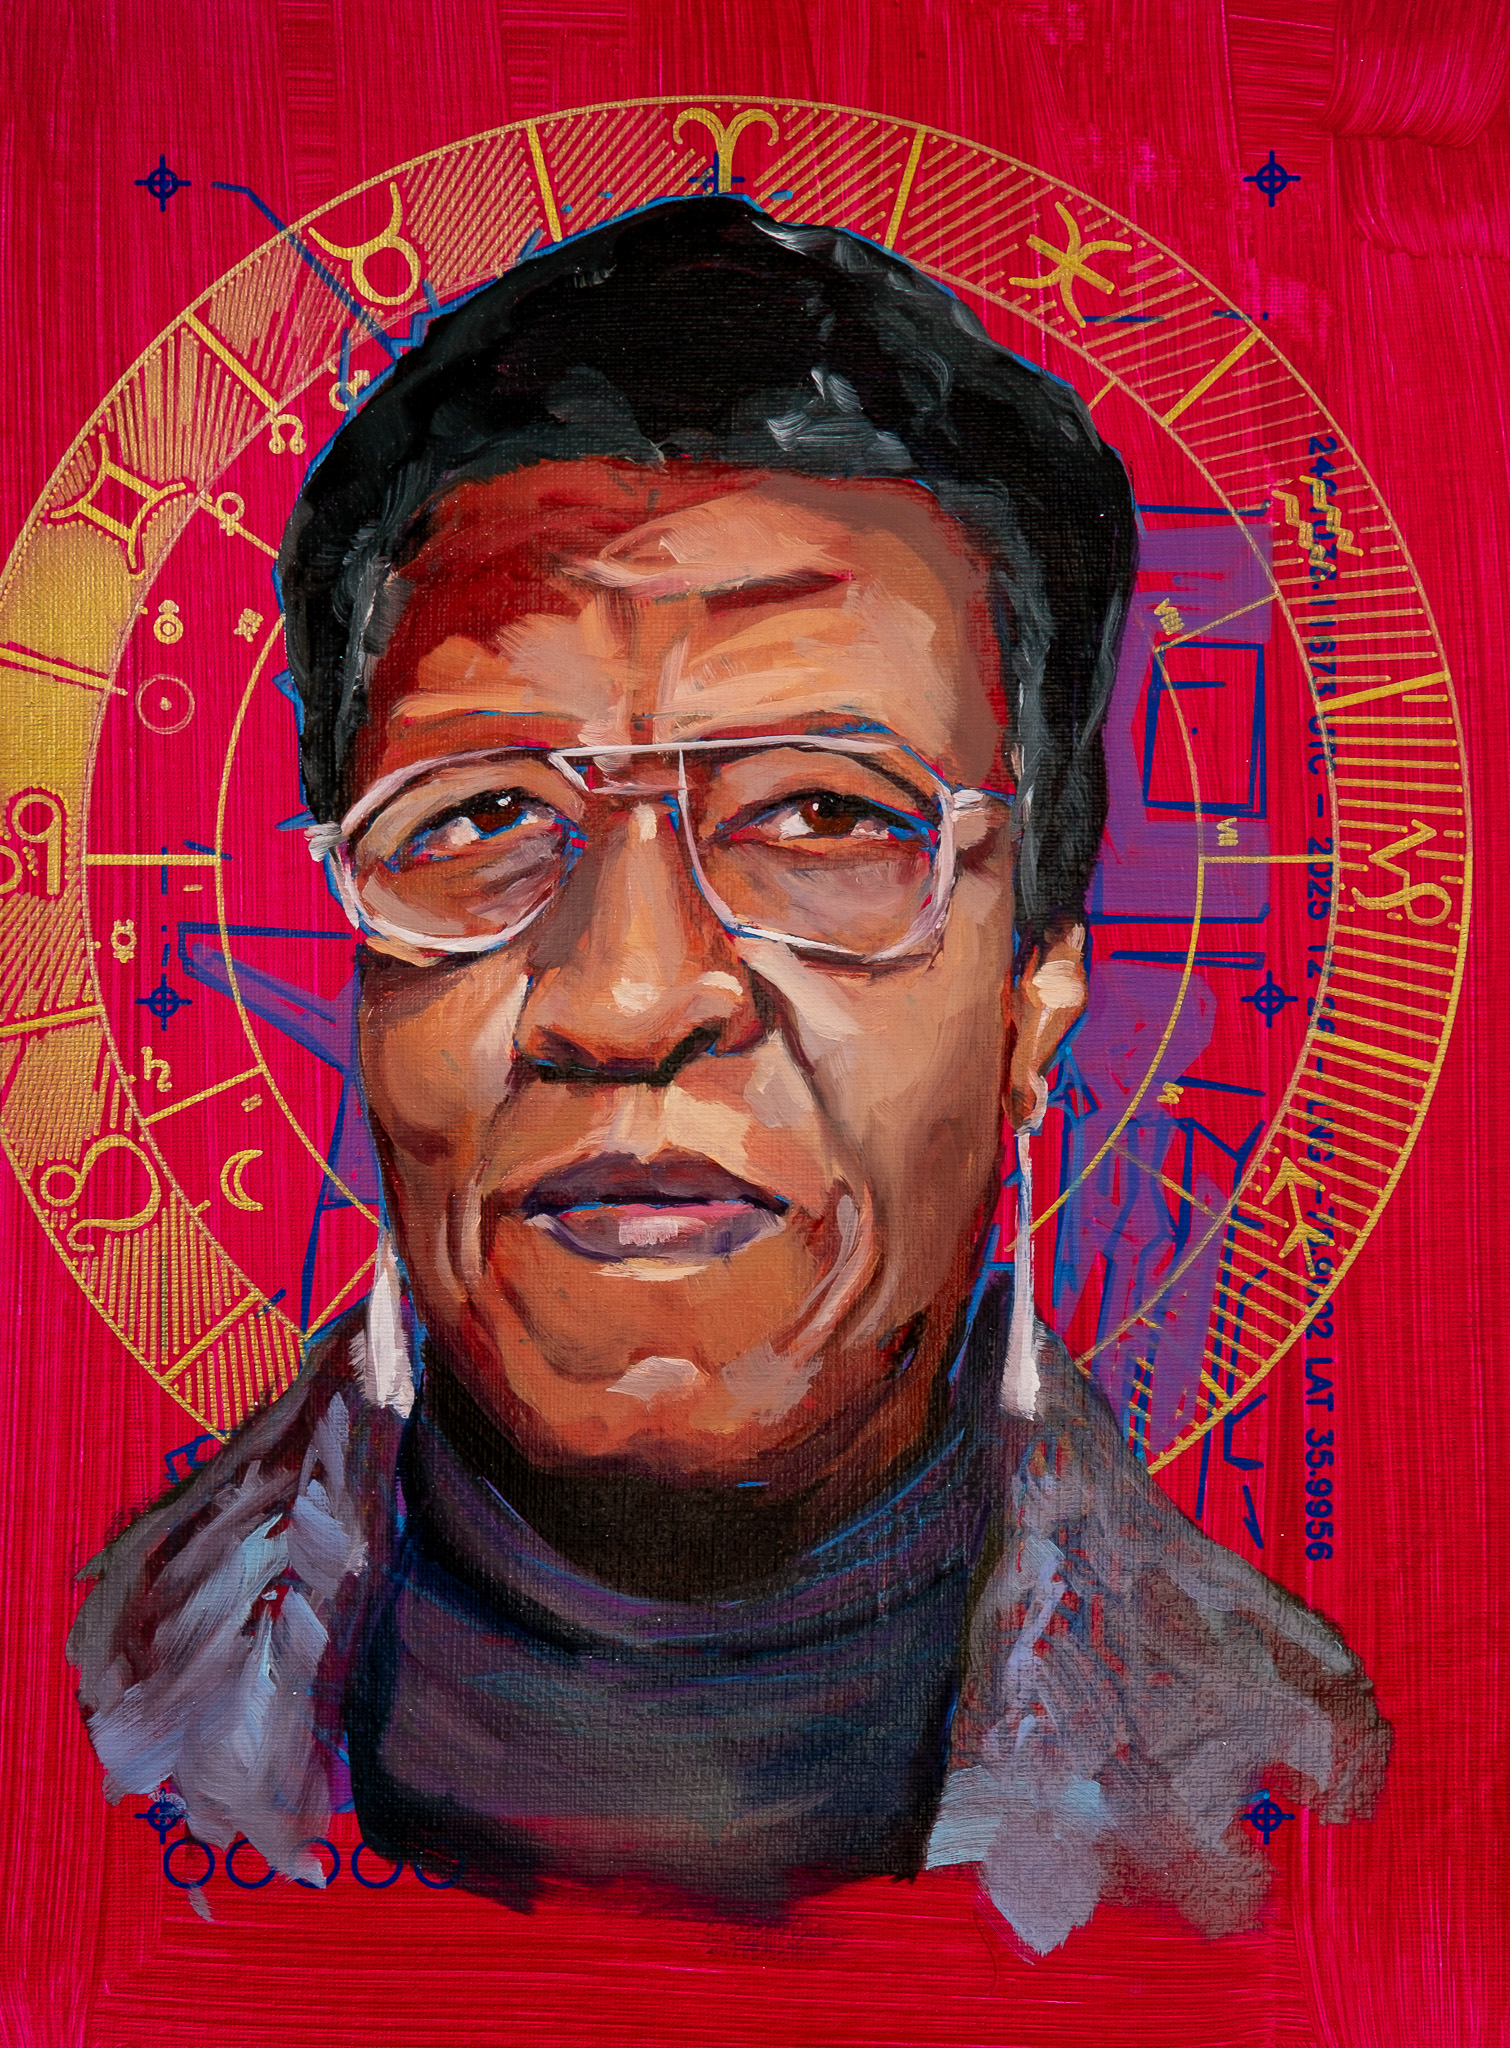
\includegraphics[width=\linewidth,height=\textheight,keepaspectratio]{2026/santos/images/DSF1039.jpg}}
\end{minipage}
\hfill
\begin{minipage}[b][\textheight][b]{0.48\textwidth}
  {\renewcommand{\arraystretch}{1.0}\setstretch{1.0}\selectfont
\begin{tabular}[b]{@{}l@{}}
Octavia, 2025\\
Oil on canvas\\
16 x 12 inches
\end{tabular}}
\end{minipage}%
}%
\clearpage
{\setlength{\parskip}{0pt}%
\noindent
\begin{minipage}[b][\textheight][b]{0.48\textwidth}
  \hfill{\renewcommand{\arraystretch}{1.0}\setstretch{1.0}\selectfont
\begin{tabular}[b]{@{}r@{}}
David, 2026\\
Oil on canvas\\
16 x 12 inches
\end{tabular}}
\end{minipage}
\hfill
\begin{minipage}[b][\textheight][b]{0.48\textwidth}
  \href{https://patriciogonzalezvivo.com/2026/santos/#DSF1040}{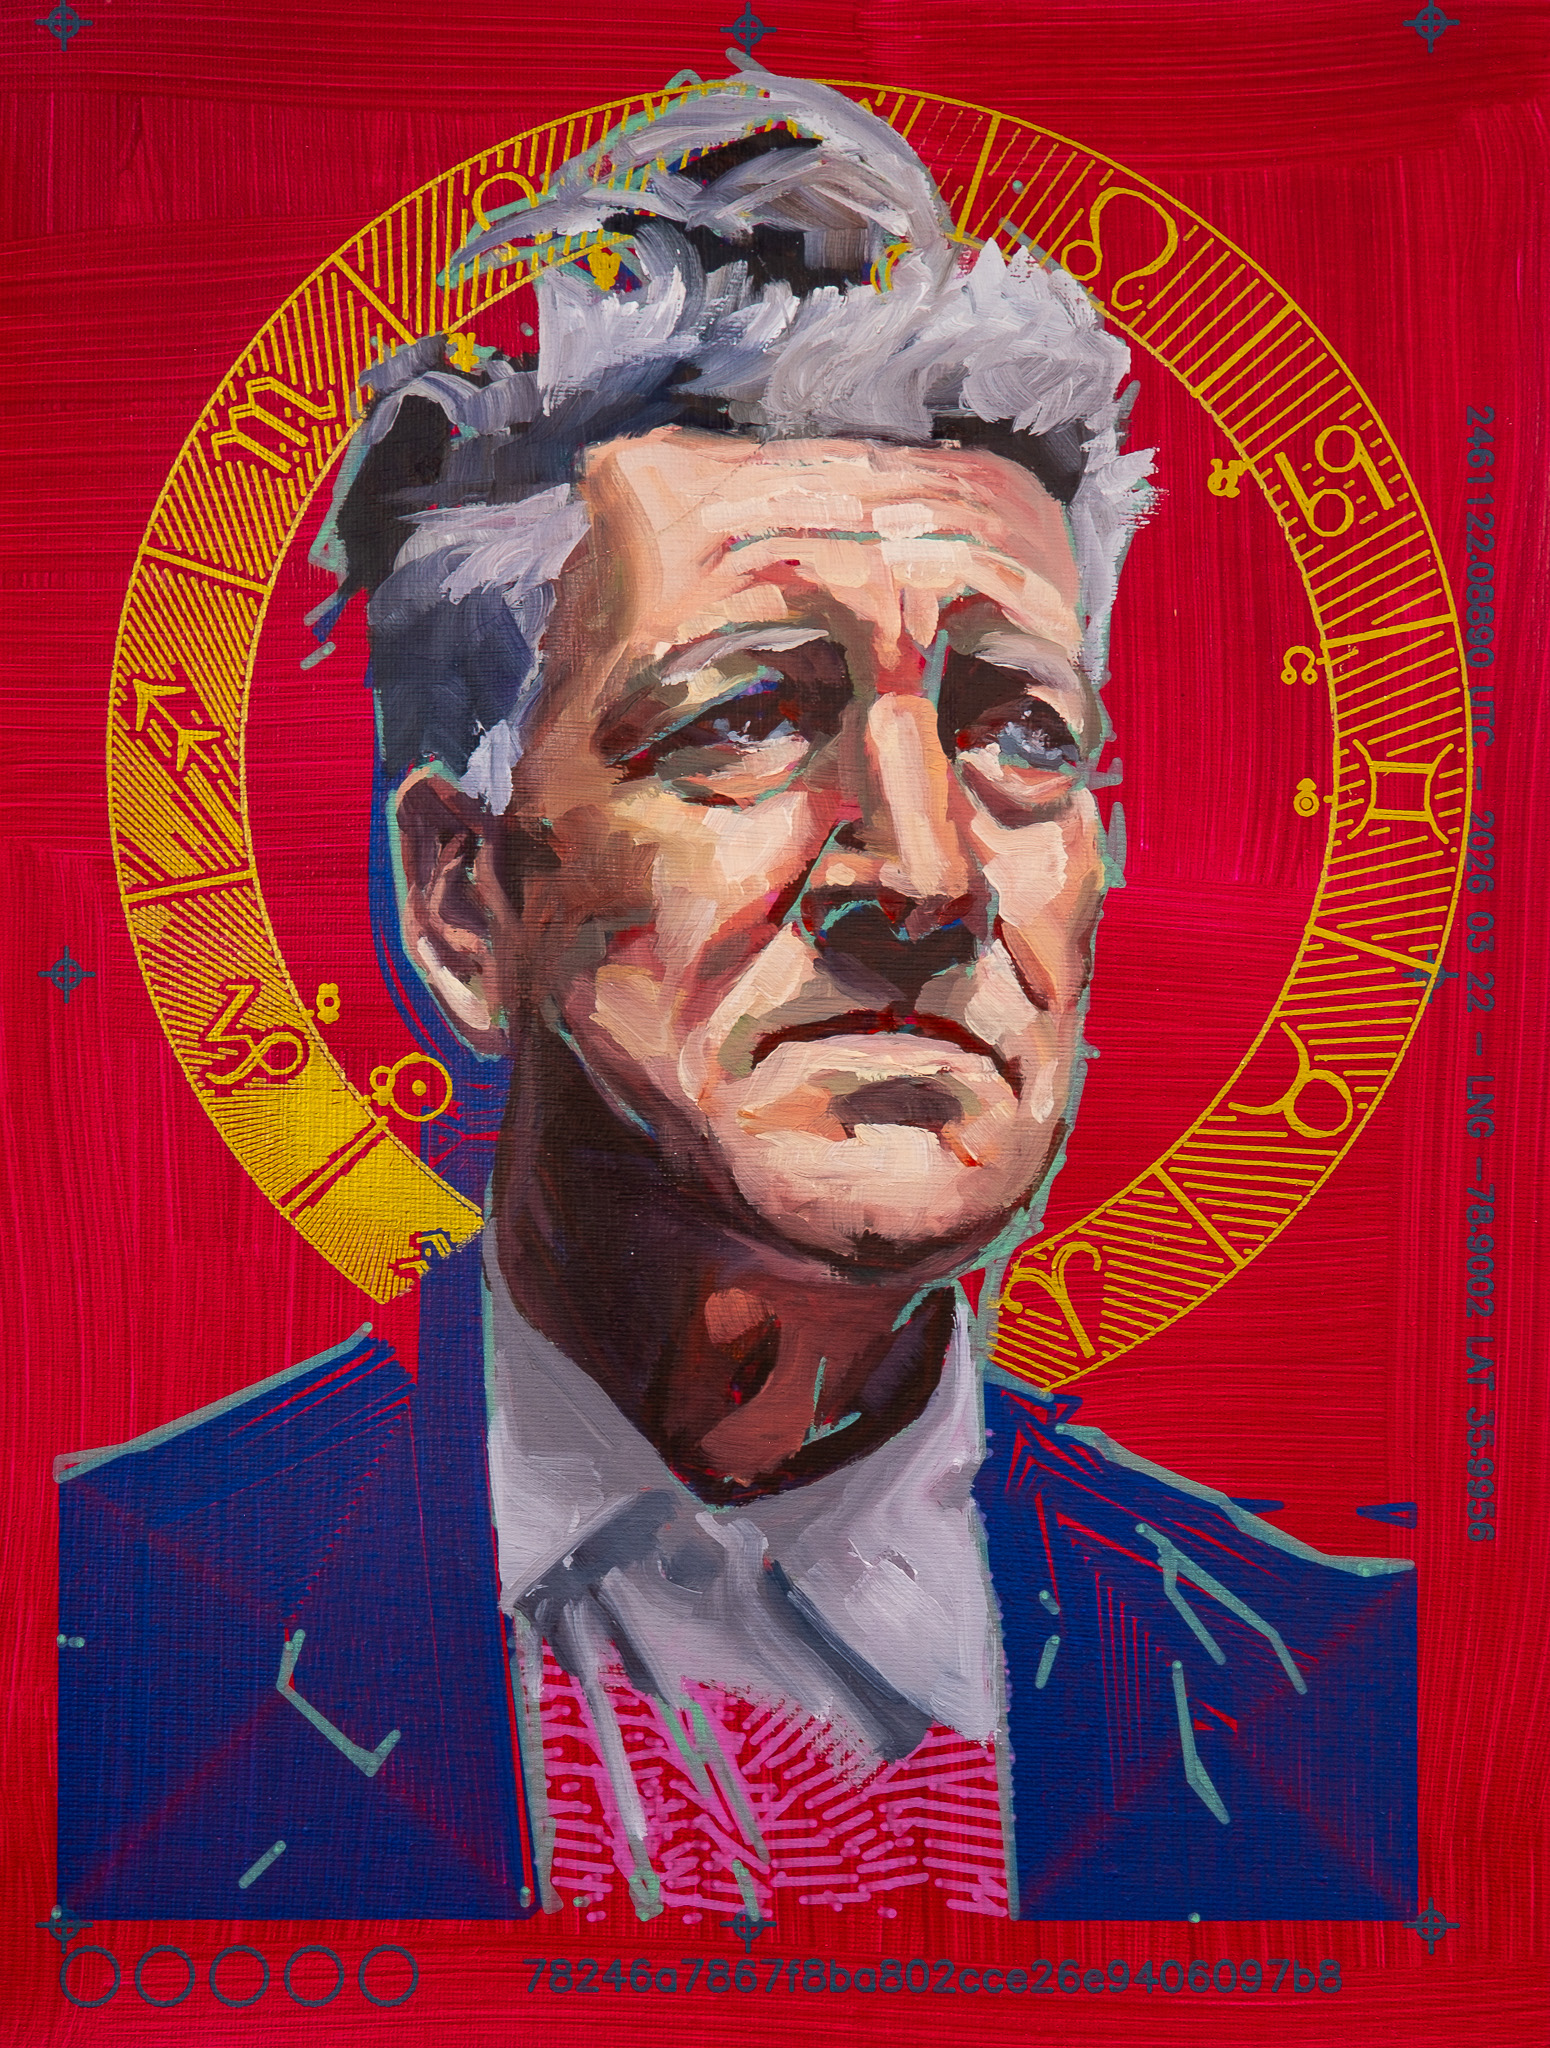
\includegraphics[width=\linewidth,height=\textheight,keepaspectratio]{2026/santos/images/DSF1040.jpg}}
\end{minipage}%
}%
\clearpage
{\setlength{\parskip}{0pt}%
\noindent
\begin{minipage}[b][\textheight][b]{0.48\textwidth}
  \hfill\href{https://patriciogonzalezvivo.com/2026/santos/#DSF1043}{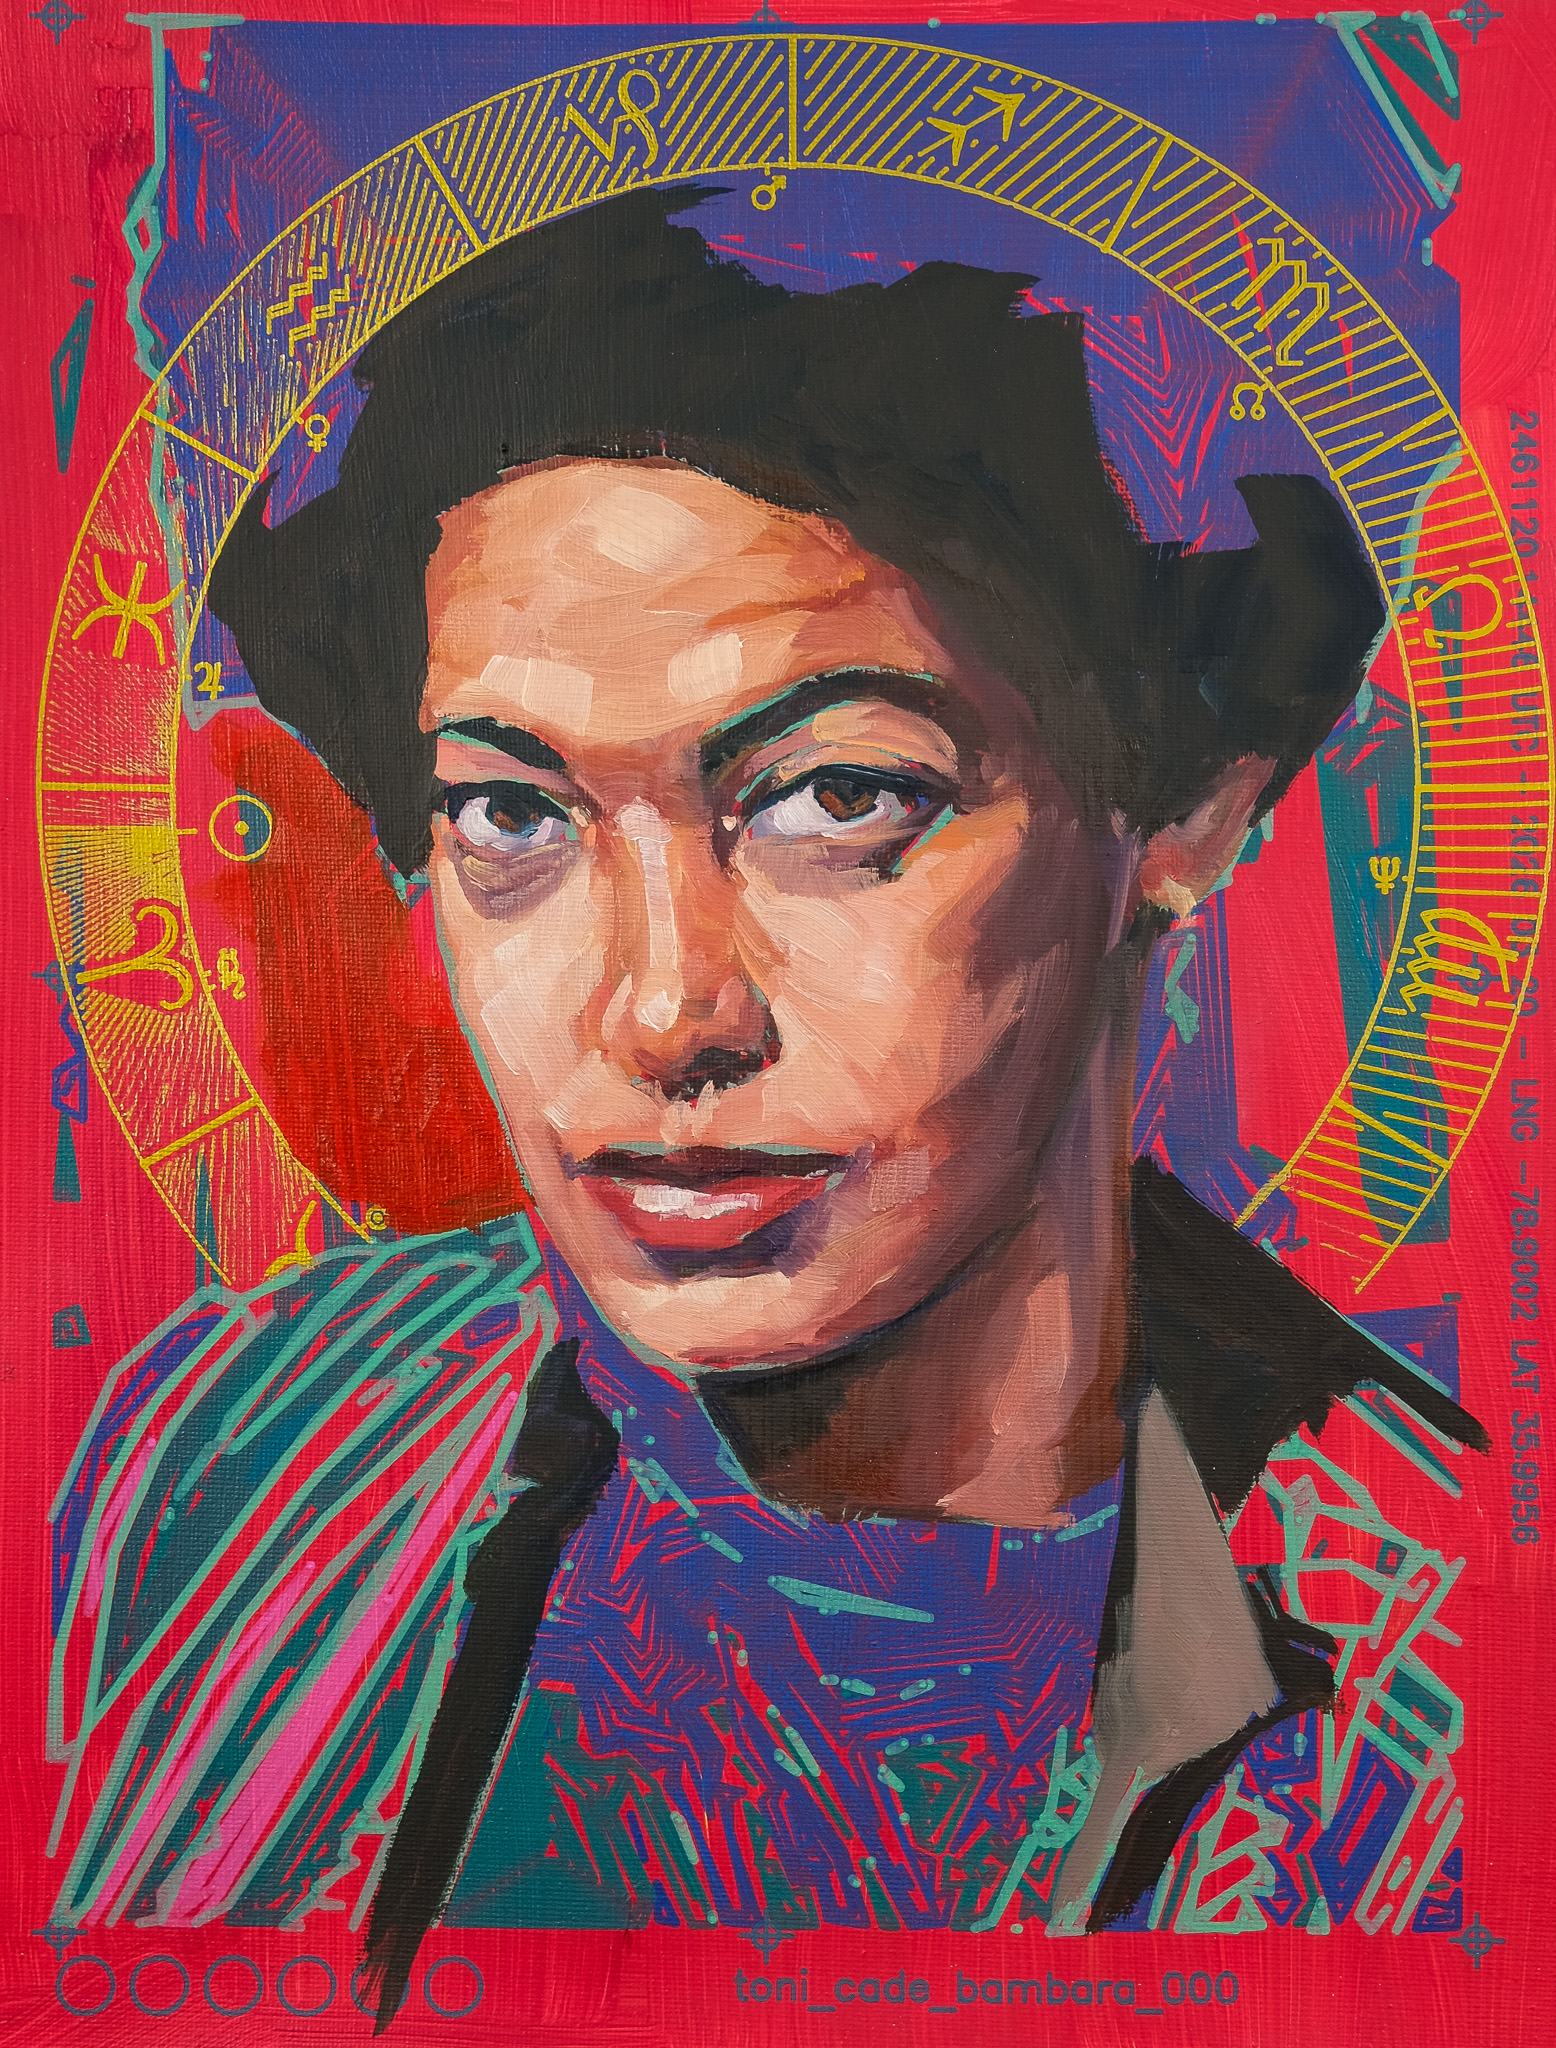
\includegraphics[width=\linewidth,height=\textheight,keepaspectratio]{2026/santos/images/DSF1043.jpg}}
\end{minipage}
\hfill
\begin{minipage}[b][\textheight][b]{0.48\textwidth}
  {\renewcommand{\arraystretch}{1.0}\setstretch{1.0}\selectfont
\begin{tabular}[b]{@{}l@{}}
Toni, 2026\\
Oil on canvas\\
16 x 12 inches
\end{tabular}}
\end{minipage}%
}%
\clearpage
{\setlength{\parskip}{0pt}%
\noindent
\begin{minipage}[b][\textheight][b]{0.48\textwidth}
  \hfill{\renewcommand{\arraystretch}{1.0}\setstretch{1.0}\selectfont
\begin{tabular}[b]{@{}r@{}}
Lygia, 2026\\
Oil on canvas\\
16 x 12 inches
\end{tabular}}
\end{minipage}
\hfill
\begin{minipage}[b][\textheight][b]{0.48\textwidth}
  \href{https://patriciogonzalezvivo.com/2026/santos/#DSF1045}{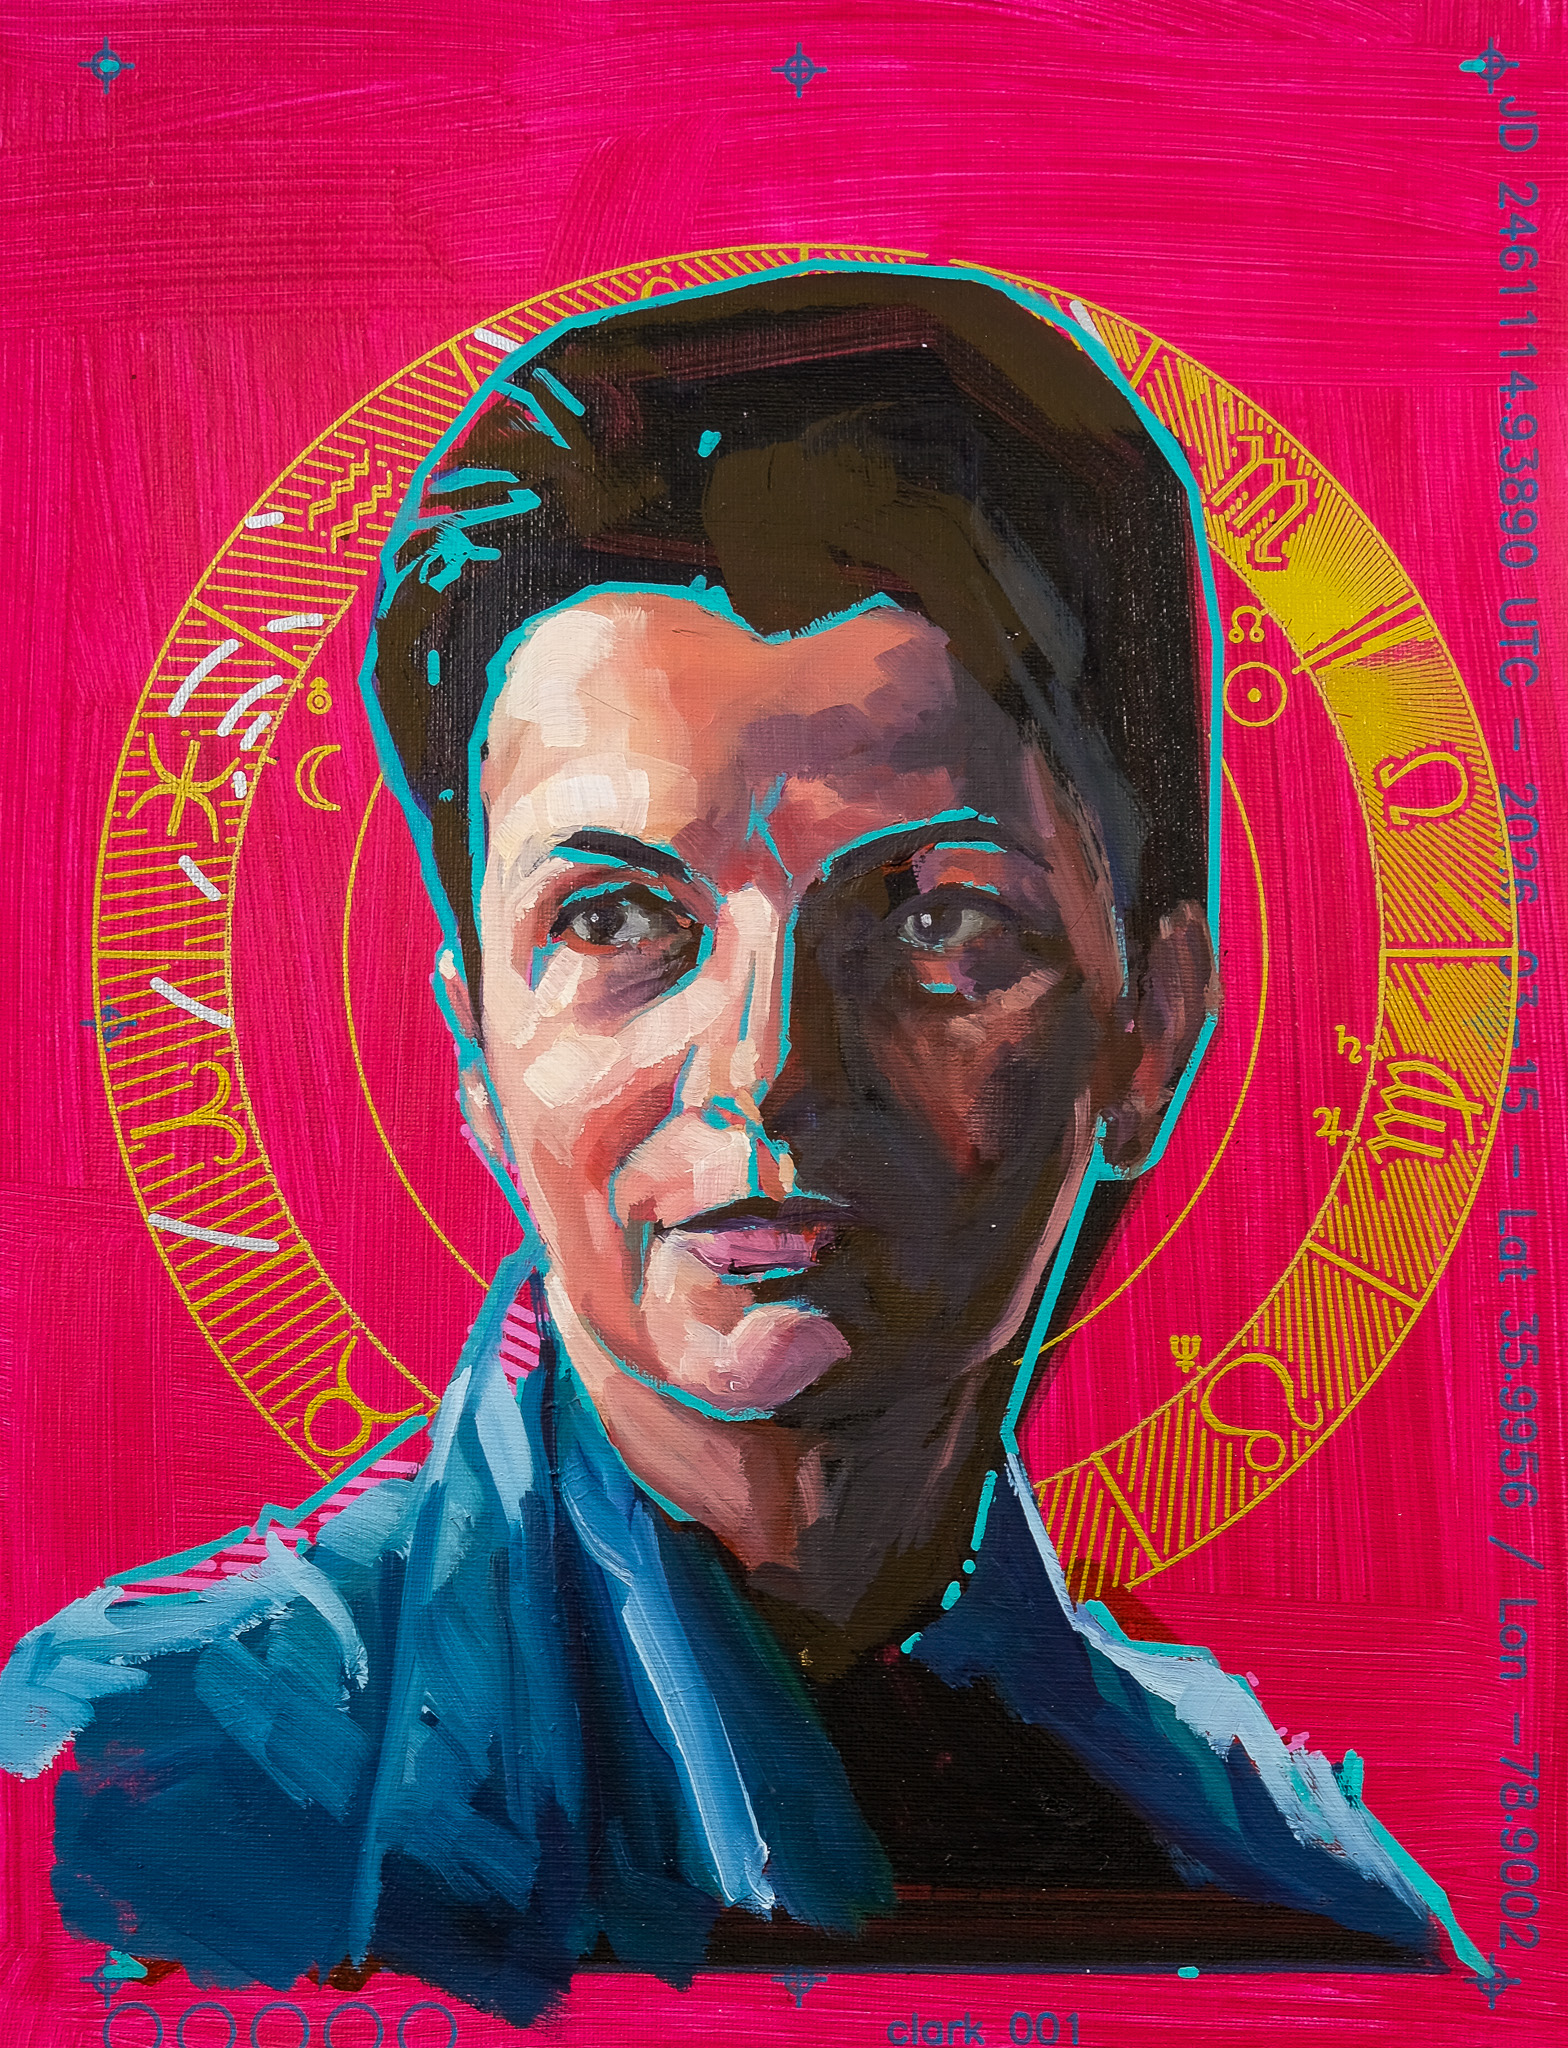
\includegraphics[width=\linewidth,height=\textheight,keepaspectratio]{2026/santos/images/DSF1045.jpg}}
\end{minipage}%
}%
\clearpage
{\setlength{\parskip}{0pt}%
\noindent
\begin{minipage}[b][\textheight][b]{0.48\textwidth}
  \hfill\href{https://patriciogonzalezvivo.com/2026/santos/#DSF1047}{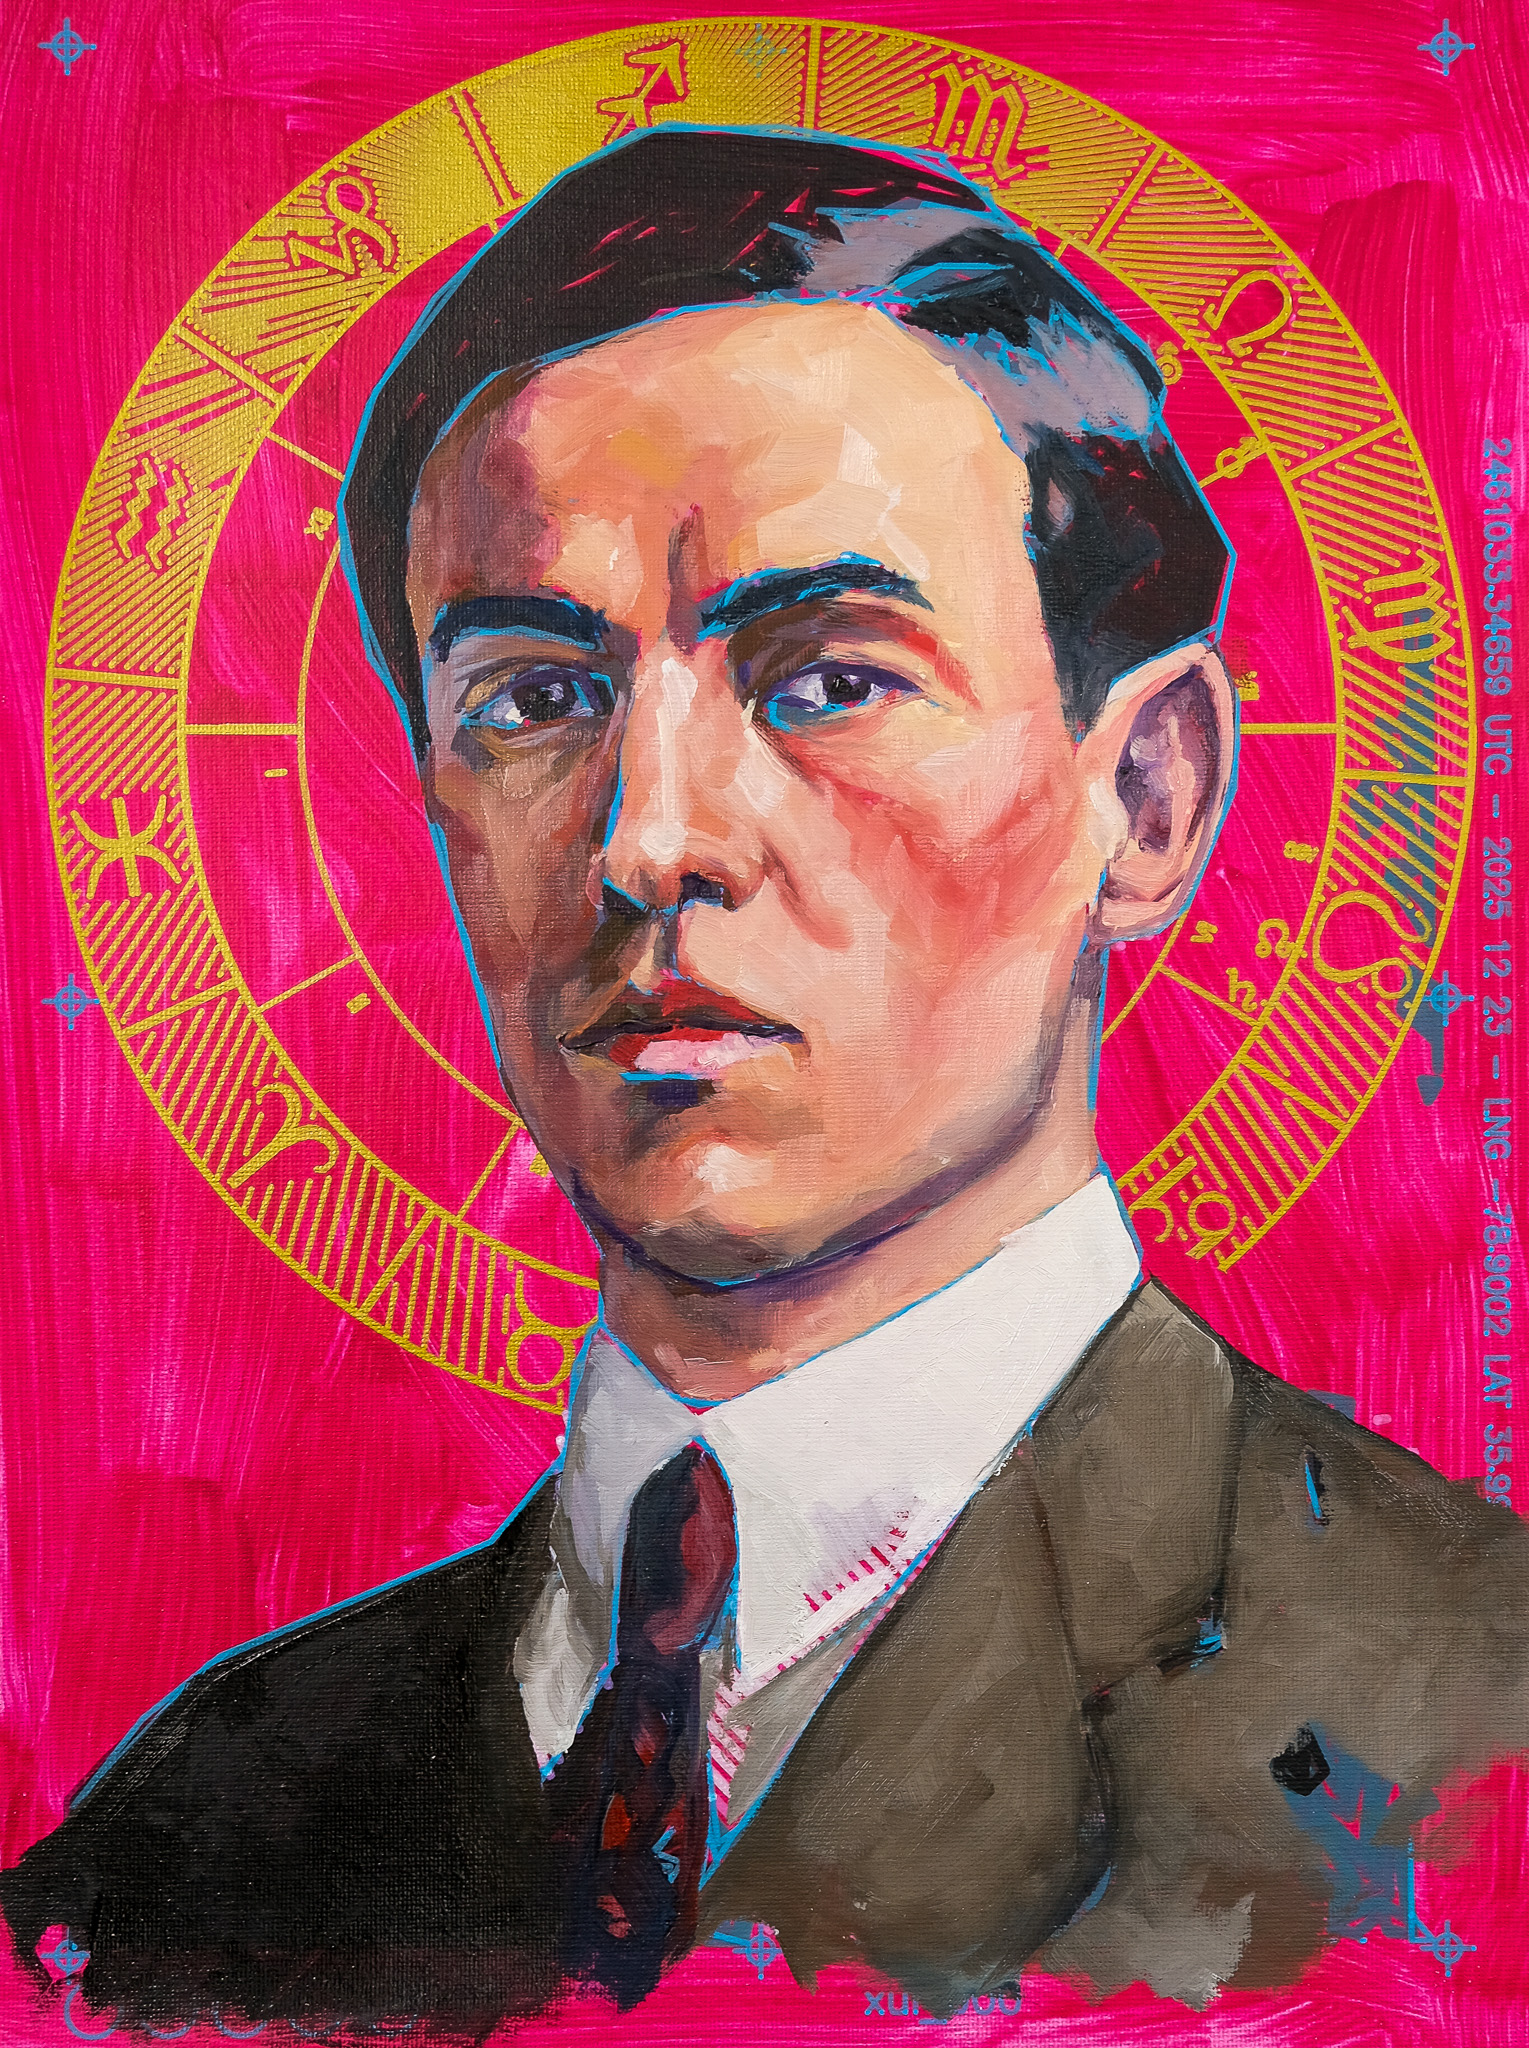
\includegraphics[width=\linewidth,height=\textheight,keepaspectratio]{2026/santos/images/DSF1047.jpg}}
\end{minipage}
\hfill
\begin{minipage}[b][\textheight][b]{0.48\textwidth}
  {\renewcommand{\arraystretch}{1.0}\setstretch{1.0}\selectfont
\begin{tabular}[b]{@{}l@{}}
Xul, 2025\\
Oil on canvas\\
16 x 12 inches
\end{tabular}}
\end{minipage}%
}%

\clearpage
\markright{\href{https://patriciogonzalezvivo.com/2026/weaver2/}{Weaver}, 2025-2026}
\noindent{\Large\textbf{\href{https://patriciogonzalezvivo.com/2026/weaver2/}{Weaver}}}\hfill{\large \href{https://patriciogonzalezvivo.com/2025-2026/}{\textcolor{red}{2025-2026}}}

\begin{wrapfigure}{r}{0.40\textwidth}
\vspace{-\intextsep}
\noindent\hfill \href{https://patriciogonzalezvivo.com/2026/weaver2/}{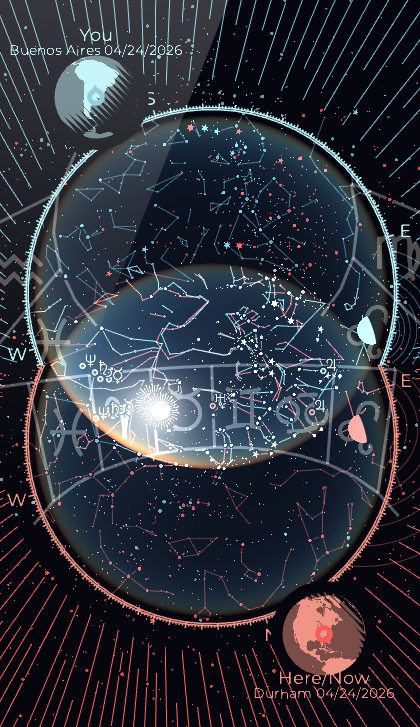
\includegraphics[width=\linewidth,height=0.75\textheight,keepaspectratio]{2026/weaver2/thumbnail.jpg}}
\vspace{-\intextsep}
\end{wrapfigure}
\begin{wrapfigure}{l}{0.40\textwidth}
\vspace{-\intextsep}
\includegraphics[width=\linewidth,keepaspectratio]{temp_portfolio/html_renders/looom_000_light_f0.png}
\vspace{-\intextsep}
\end{wrapfigure}


In the middle of the nineteenth century, during the Great Potato Famine, Dudley Sarsfield Brennan (b. 1810, Ireland) and Mary Colcough (b. 1826, Ireland) left their homeland and crossed the Atlantic toward Argentina. The voyage lasted between four to six months, likely beginning on early summer. At the time, such journeys were long and unforgiving.

I imagine them walking the deck at night beneath an open sky, breathing the cold ocean air. As the ship moved southward, familiar constellations slowly disappeared beyond the northern horizon while unknown stars emerged from the southern sky. I imagine them speaking quietly, sometimes in conversation, sometimes in silence, wondering about the life awaiting them across the ocean. I feel in them a mixture of grief and hope: the awareness of being small and transient beneath the immensity of the universe. A metal ship crossing a dark sea on a planet spinning around a sun, itself drifting through space.

Eventually they arrived in Buenos Aires and settled in the town of Magdalena, where their only child, Patricio, was born in 1870.

More than twenty years later, Enrico Vivo (b. 1868, Italy) and Maria Viva (b. 1870, Italy), also driven by hunger and the search for a better future, made a similar passage from the island of Anacapri to Argentina. These two couples never met, yet they shared the experience of migration and became part of the same lineage.

From my paternal family I inherited the name Patricio; from my maternal family, the surname Vivo. I stand at the far end of their horizon, beneath a different sky from the one that greeted them in Buenos Aires. My lineage is one of voyagers, nomads, and wanderers. I long to connect with them, yet all I possess are fragments of their stories and the sky itself.

From this desire, I created Weaver: a way of threading my present to their future, my past to their present. A way of seeing what they saw, and of allowing future generations to see what I see.

--- 

\begin{wrapfigure}{r}{0.40\textwidth}
\vspace{-\intextsep}
\includegraphics[width=\linewidth,keepaspectratio]{temp_portfolio/html_renders/looom_001_light_f0.png}
\vspace{-\intextsep}
\end{wrapfigure}


Weaver is an interactive work that invites two people to meet across time and space through a shared fragment of the night sky. Like a prayer or a ritual, it offers a passage beyond immediate experience into a quiet awareness of what connects us, not despite distance, but through it.

<!--  -->

Two celestial maps overlap: one for each observer. Each is rendered in a distinct color, reflecting the night sky from a specific place and moment. In the region where the maps intersect lie the constellations both participants share, a common sky that exists beyond distance or time.

Each map uses a polar projection. Stars near the outer edge rest close to the horizon (marked by the cardinal directions), while those at the center hover directly overhead. This perspective situates each observer within their own sky, while revealing where their visions align.

<!--  -->

Beside each map, a rotating globe marks the observer's location. Both the celestial maps and the globes are fully interactive. By dragging the sky, you can shift the date and time; by rotating the globe, you can reposition the observer anywhere on Earth.

--- 

\begin{wrapfigure}{l}{0.40\textwidth}
\vspace{-\intextsep}
\href{https://themapisnot.com/issue-iv-patricio-gonzalez-vivo-jen-lowe}{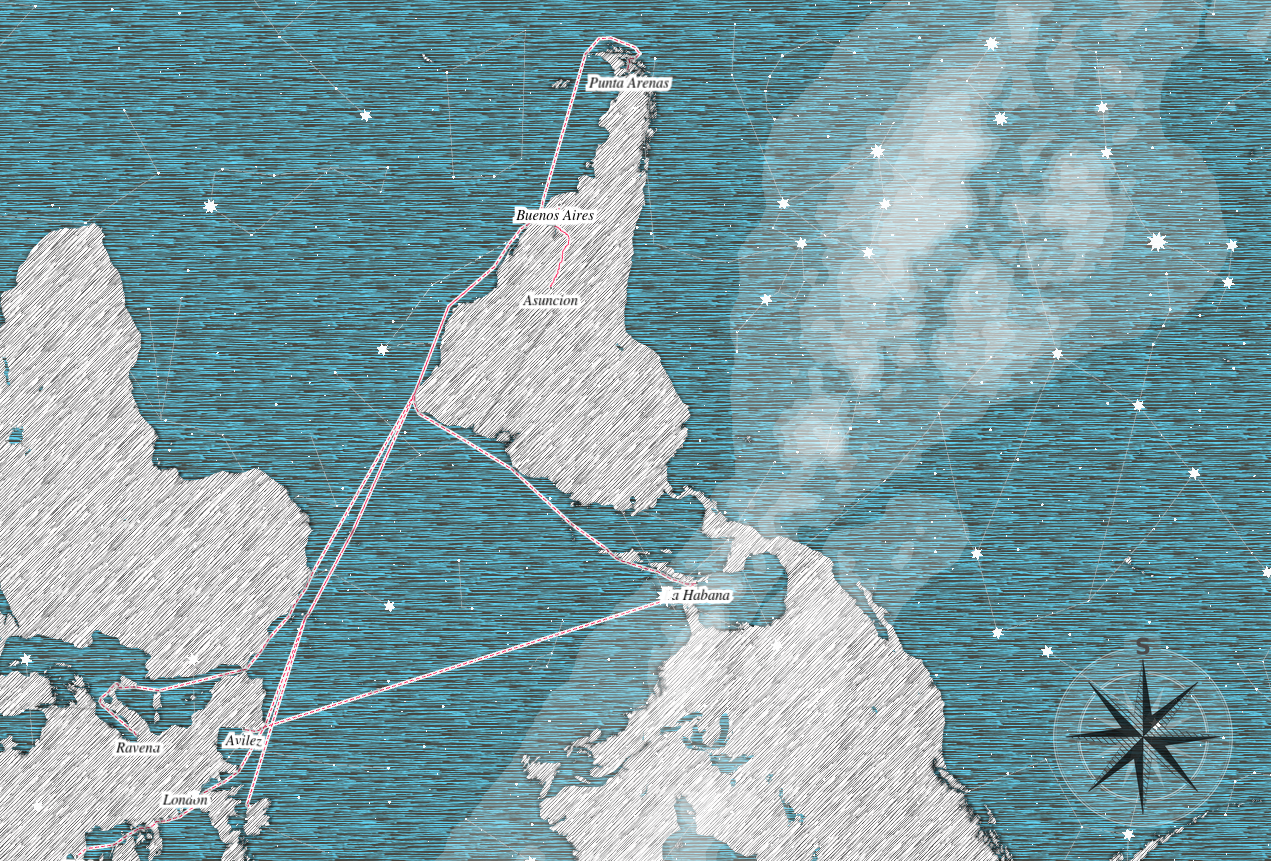
\includegraphics[width=\linewidth,keepaspectratio]{2026/weaver2/../../2017/guayupia/images/paths.png}}
\par\vspace{0.4em}
{\small \raggedright
\textbf{Guayupia}, 2017 \\
Digital map
\par}
\vspace{-\intextsep}
\end{wrapfigure}


This project continue a personal exploration of my family history and the experience of migration started with the project \href{https://themapisnot.com/issue-iv-patricio-gonzalez-vivo-jen-lowe}{\textbf{Guayupia (2017) for the digital exposition Territory}} in collaboration with \href{https://www.jenlowe.net/}{\textbf{Jen Lowe}}. 

The addition of the stars and the sky on Guaypuia was the begining of a 10 years long obsession for learning about the movement of the stars and planets. An passion that lead me to study astronomy through the creation of my own astronomical library call \href{https://github.com/patriciogonzalezvivo/hypatia}{\textbf{Hypathia}} and the creation of several artworks exploring the relationship between the sky and human awareness, such as \href{https://patriciogonzalezvivo.com/2017/luna/}{\textbf{LUNA (2017)}} and \href{https://patriciogonzalezvivo.com/2025/orbitas2/}{\textbf{Orbitas (2018)}}, \href{https://patriciogonzalezvivo.com/2018/estrellas/}{\textbf{ESTRELLAS (2018)}} and \href{https://patriciogonzalezvivo.com/2019/hogar/}{\textbf{HOGAR (2019)}}.

\clearpage
{\setlength{\parskip}{0pt}%
\noindent
\begin{minipage}[b][\textheight][c]{\textwidth}
  \centering
  \href{https://patriciogonzalezvivo.com/2026/weaver2/#000}{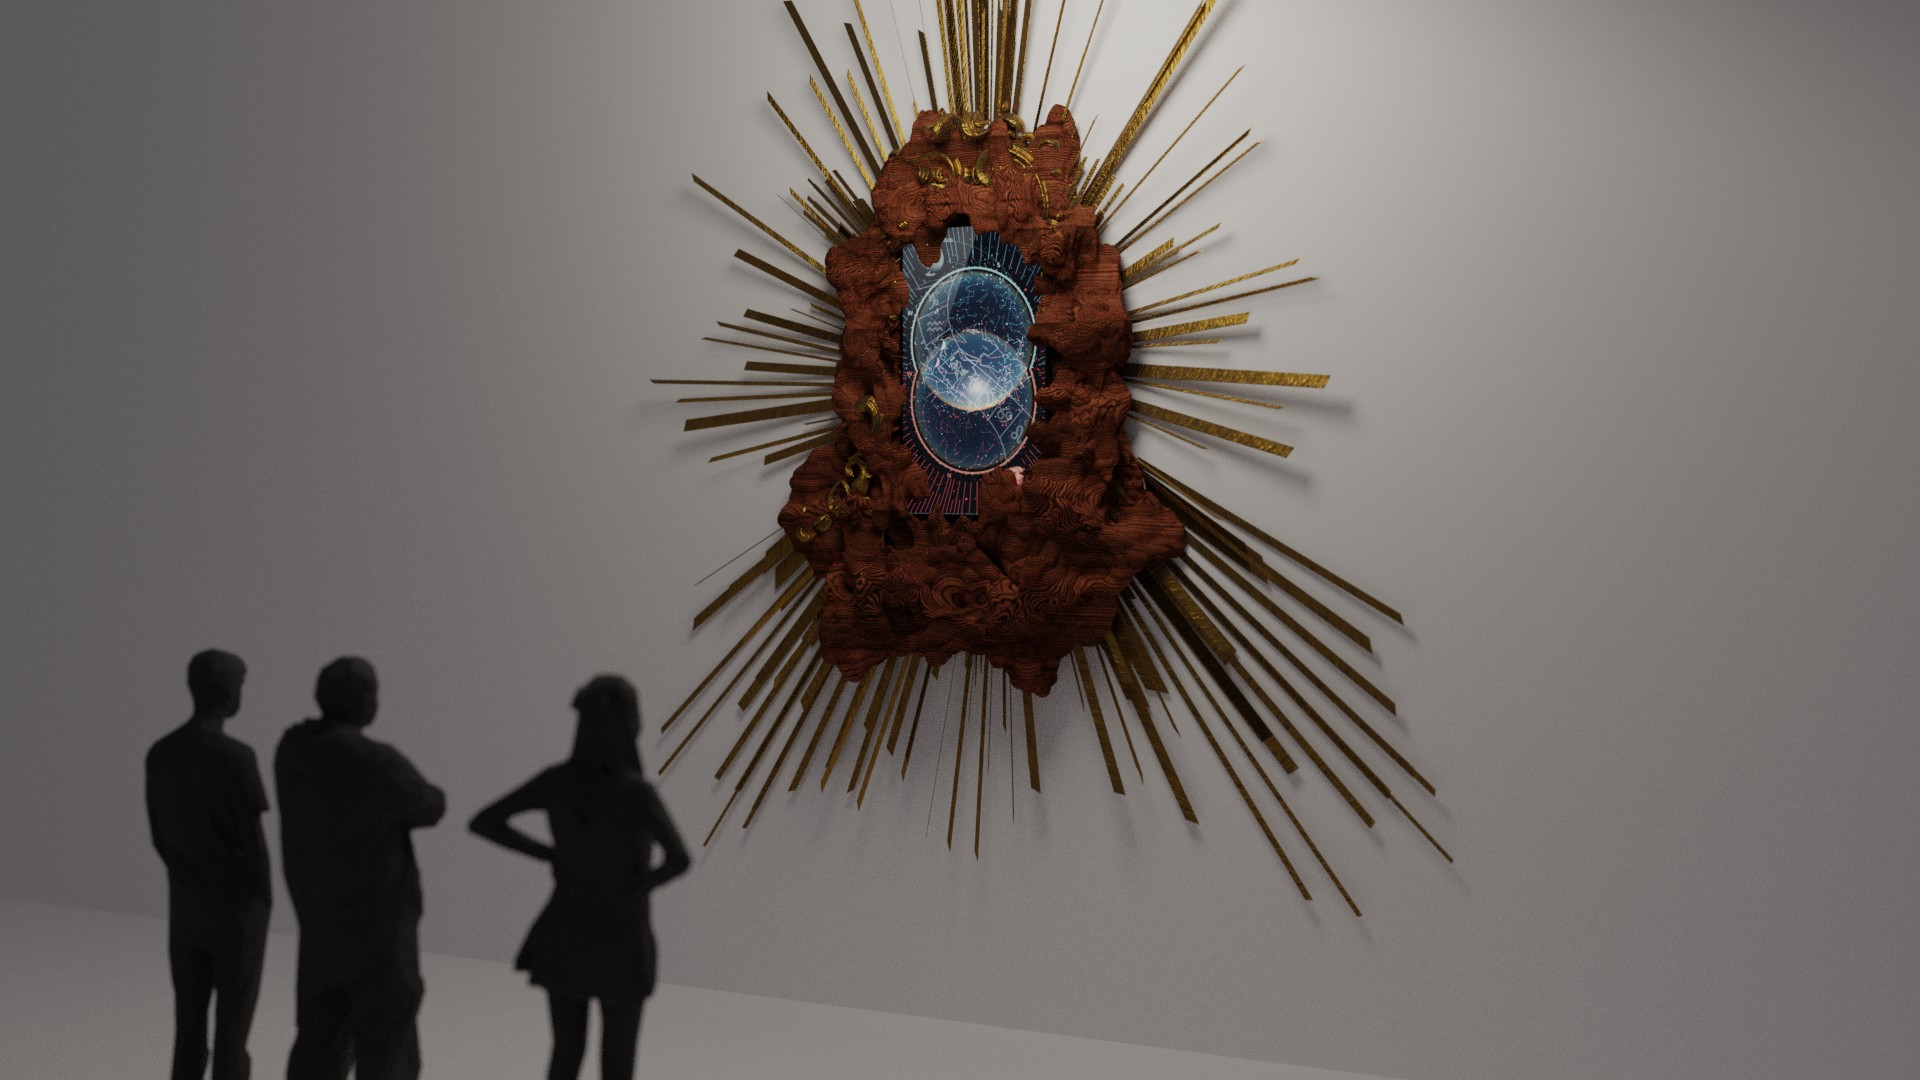
\includegraphics[width=\linewidth,height=\textheight,keepaspectratio]{2026/weaver2/images/000.jpg}}
\end{minipage}%
}%
\clearpage
{\setlength{\parskip}{0pt}%
\noindent
\begin{minipage}[b][\textheight][c]{\textwidth}
  \centering
  \href{https://patriciogonzalezvivo.com/2026/weaver2/#001}{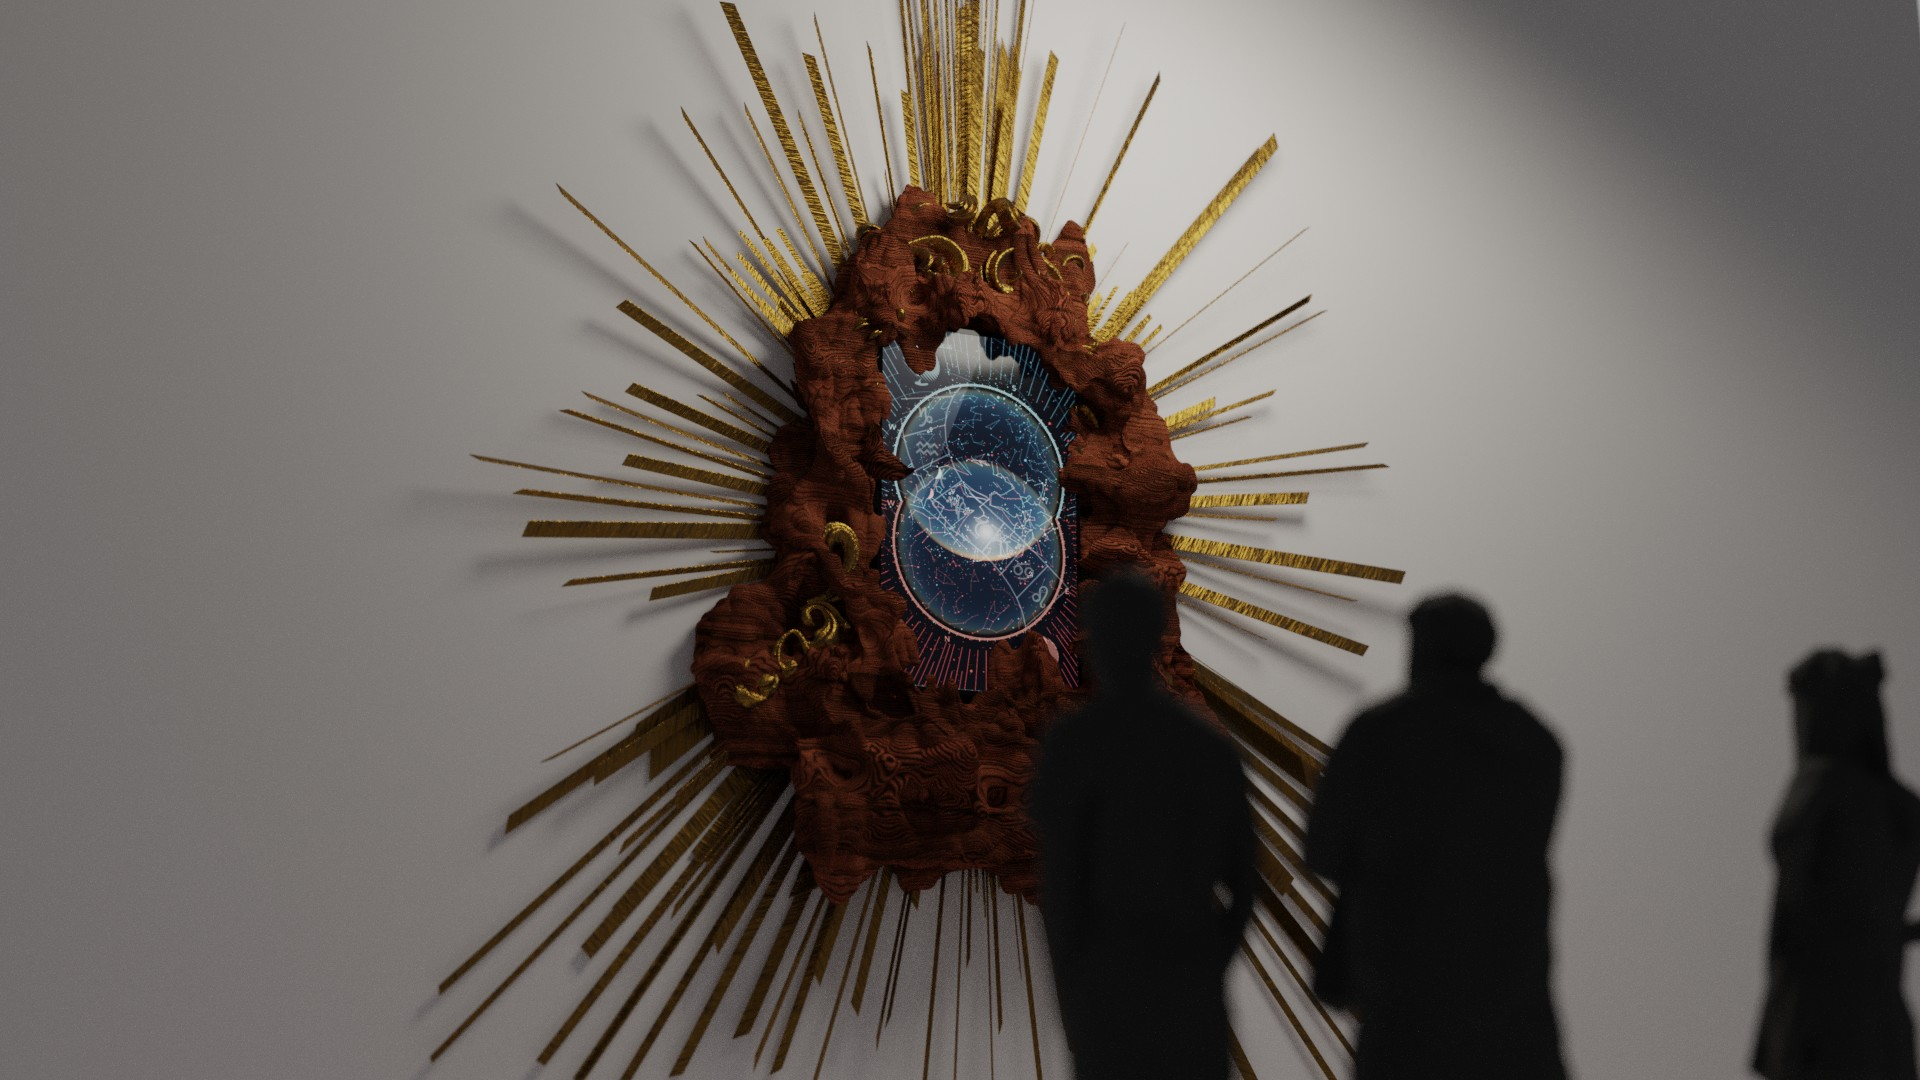
\includegraphics[width=\linewidth,height=\textheight,keepaspectratio]{2026/weaver2/images/001.jpg}}
\end{minipage}%
}%

\clearpage
\noindent{\Large\textbf{Related Works}}
\par\vspace{0.5em}\noindent\hrulefill\par\vspace{1em}
{\setlength{\parskip}{0pt}%
\noindent
\begin{minipage}[t]{0.31\textwidth}
\href{https://patriciogonzalezvivo.com/2019/hogar/}{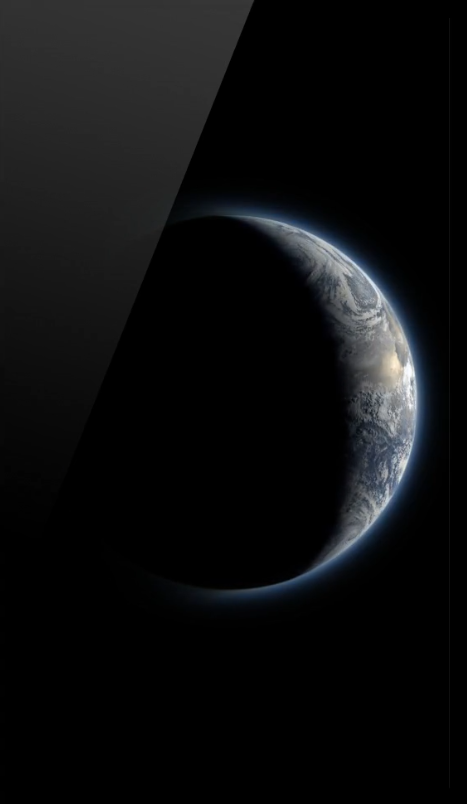
\includegraphics[width=\linewidth,height=0.72\textheight,keepaspectratio]{2019/hogar/thumbnail.png}}
\vspace{0.5em}
{\renewcommand{\arraystretch}{1.0}\setstretch{1.0}\selectfont
\begin{tabular}[b]{@{}l@{}}
Hogar, 2019\\
Custom real-time software\\
Variable dimensions
\end{tabular}}
\end{minipage}\hfill
\begin{minipage}[t]{0.31\textwidth}
\href{https://patriciogonzalezvivo.com/2018/estrellas/}{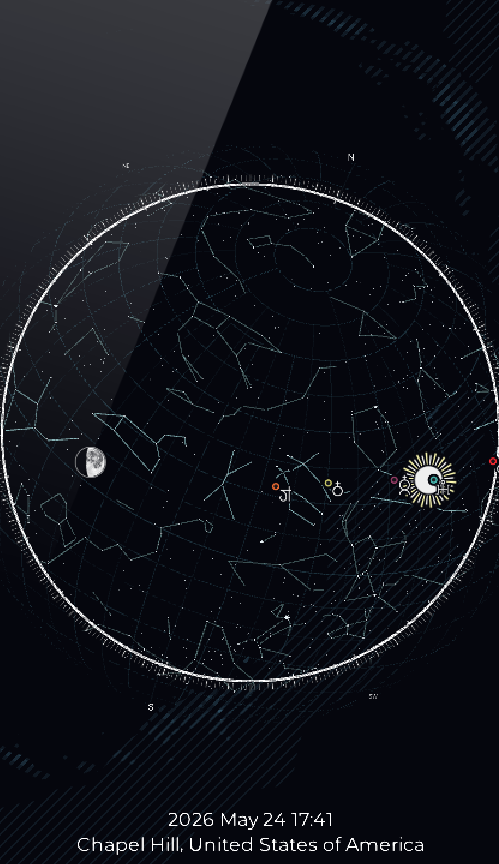
\includegraphics[width=\linewidth,height=0.72\textheight,keepaspectratio]{2018/estrellas/thumbnail.png}}
\vspace{0.5em}
{\renewcommand{\arraystretch}{1.0}\setstretch{1.0}\selectfont
\begin{tabular}[b]{@{}l@{}}
Estrellas, 2018\\
Custom real-time software\\
Variable dimensions
\end{tabular}}
\end{minipage}\hfill
\begin{minipage}[t]{0.31\textwidth}
\href{https://patriciogonzalezvivo.com/2017/luna/}{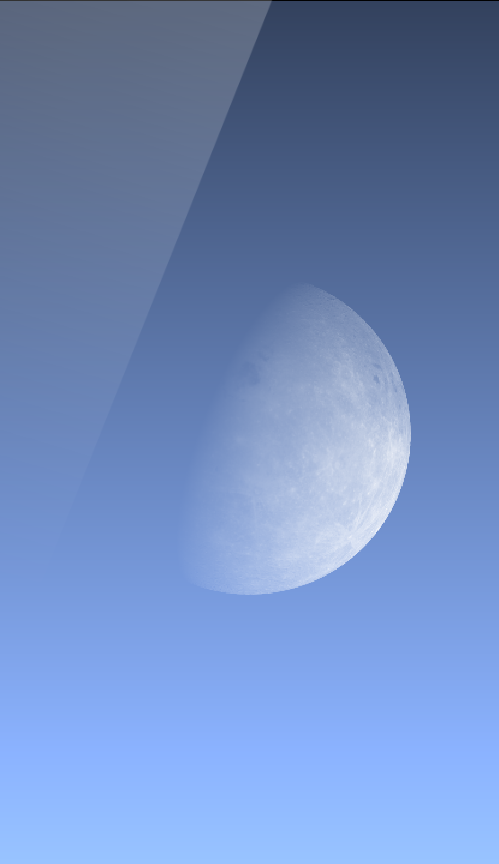
\includegraphics[width=\linewidth,height=0.72\textheight,keepaspectratio]{2017/luna/thumbnail.png}}
\vspace{0.5em}
{\renewcommand{\arraystretch}{1.0}\setstretch{1.0}\selectfont
\begin{tabular}[b]{@{}l@{}}
Luna, 2017\\
Custom real-time software\\
Variable dimensions
\end{tabular}}
\end{minipage}
}%

\clearpage









% ---------------------------------------------------------
% CONTACT PAGE
% ---------------------------------------------------------
\clearpage
\markright{Contact}

% \noindent
% \begin{minipage}[t]{0.15\textwidth}
% \vspace{0pt}
% 
\includegraphics[width=\linewidth,keepaspectratio]{images/logo-gray.png}
% \end{minipage}%
% \hfill
\begin{minipage}[t]{0.50\textwidth}
\vspace{0.3in}
\raggedright
\begin{tabular}{rl}
% \textbf{Name}:     & Patricio Gonzalez Vivo     \\
\textbf{Location} & 1234 Street, City, Country \\
\textbf{Phone}    & +1 415 999 9999    \\
\textbf{Email}    & \href{mailto:patriciogonzalezvivo@gmail.com}{patriciogonzalezvivo@gmail.com} \\
\textbf{Web}      & \href{https://patriciogonzalezvivo.com}{patriciogonzalezvivo.com} \\
\textbf{Instagram} & \href{https://instagram.com/patriciogonzalezvivo}{@patriciogonzalezvivo} \\
\end{tabular}
\end{minipage}%
\hfill
\begin{minipage}[t]{0.25\textwidth}
\vspace{0pt}
\raggedleft

\includegraphics[width=\linewidth,keepaspectratio]{images/qr-code.png}
\end{minipage}

\vspace{1cm}

% =========================================================
% END DOCUMENT
% =========================================================
\end{document}
